%
% Remi Beges PhD final report
%

% Page creation engine
\documentclass[11pt,a4paper]{book}
\usepackage[utf8x]{inputenc}
\usepackage[english]{babel}
\usepackage[T1]{fontenc}

% Main modules
\usepackage{url}      % URL
\usepackage{graphicx} % Pictures
\usepackage{wrapfig}  % In-line Pictures
\usepackage{verbatim} % Code
\usepackage{mathtools,amssymb}
%\usepackage{moreverb} % Encoding
%\usepackage{listing}
\usepackage{minted}   % Code
%\usepackage{color}    % Highlight
\usepackage{xcolor}   % Color text
\usepackage{textgreek}% Greek language
\usepackage{booktabs} % Tables
\usepackage[table,xcdraw]{xcolor} % For colors in tables
\usepackage{colortbl} % For coloring rows, columns of table
\usepackage[toc,page]{appendix} % For managing appendix sections cleanly
\usepackage{algpseudocode} % For displaying pseudo-code
\usepackage{amsmath,empheq} % Math equations
\usepackage[nomain,acronym,xindy,toc]{glossaries}
\usepackage{makeidx}  % index support
\usepackage[ED=GEET-Elec, Ets=UT3]{tlsflyleaf} % Document cover
\usepackage{caption}     % float env with page breaks
\usepackage{hyperref}    % Links

\newenvironment{code}{\captionsetup{type=listing}}{}

% Glossary
\loadglsentries{./src/glos}
\makeglossaries
\makeindex

% Front page

% Meta-data
\title{Development of analysis and prediction methods for operating ESD robustness}
\author{Rémi Bèges}
\defencedate{01/01/2017}
\lab{Laboratoire d'analyse et d'architecture des systems (UMR ?)}

% PhD mentors

\nboss{3}
\makesomeone{boss}{1}{Fabrice Caignet}{}{}
\makesomeone{boss}{2}{Patrice Besse}{}{}
\makesomeone{boss}{3}{Marise Bafleur}{}{}

% PhD Defence meta-data
%% Referee
\nreferee{2}
\makesomeone{referee}{1}{First referee}{}{}
\makesomeone{referee}{2}{Second referee}{}{}
%% Judges
\njudge{5}
\makesomeone{judge}{1}{First member}{Teacher ? }{Jury President}
\makesomeone{judge}{2}{Second MEMBRE}{?}{Jury Member}
\makesomeone{judge}{3}{?}{?}{Membre du Jury}
\makesomeone{judge}{4}{?}{?}{Membre du Jury}
\makesomeone{judge}{5}{?}{?}{Membre du Jury}

% Document
\begin{document}

\makeflyleaf

\tableofcontents

% Code highlighting styles
%\lstdefinestyle{veriloga-style}{
  language=Verilog,
  basicstyle=\footnotesize\ttfamily,
  commentstyle=\itshape\color{violet},
  identifierstyle=\color{blue},
  morekeywords={ border, buildmesh, cos, dx, dy, fespace, fill, func,
    int2d, label, mesh, on, pi, plot, problem, sin, real, x, y},
  % float,
  frame=single,
  numbers=left
}


\chapter{Introduction}

% Trends of the electronic field is size reduction
Electronic circuits become more miniaturized year after year.
Size reduction of integrated circuits reduces manufacturing cost per chip thanks to the increased volume.
Diminishing the size and amount of electronic devices decreases the weight of embedded systems.
In automotive for instance, this results in lowered fuel consumption and impact on the environment.
Miniaturization offers increased performance and capabilities.
More functions can be packed in the same volume.

% How is size reduced
For integrated circuits, this trend is accomplished by decreasing integrated technology size.
Any integrated technology is defined by the dimensions and shapes of fundamental electronic bricks it provides.
Those bricks are most of the time different kinds of transistors, resistors and capacitors.
The size of a technology is the smallest dimension for the smallest transistor gate, called \textlambda.
The value of \textlambda{} is essential and determines the size, power consumption, switching speed, performance and many other characteristics of the complete chip.
Until recently, Moore's law successfully predicted that technology dimensions will be reduced by a factor of two every 18 months.
The automotive world follows this trend as well, moving recently to 16nm technology nodes (see Fig. \ref{fig:nxp-techno-increase}) \cite{evolution_technologies} that are normally employed in less demanding applications.

\begin{figure}[!h]
  \centering
  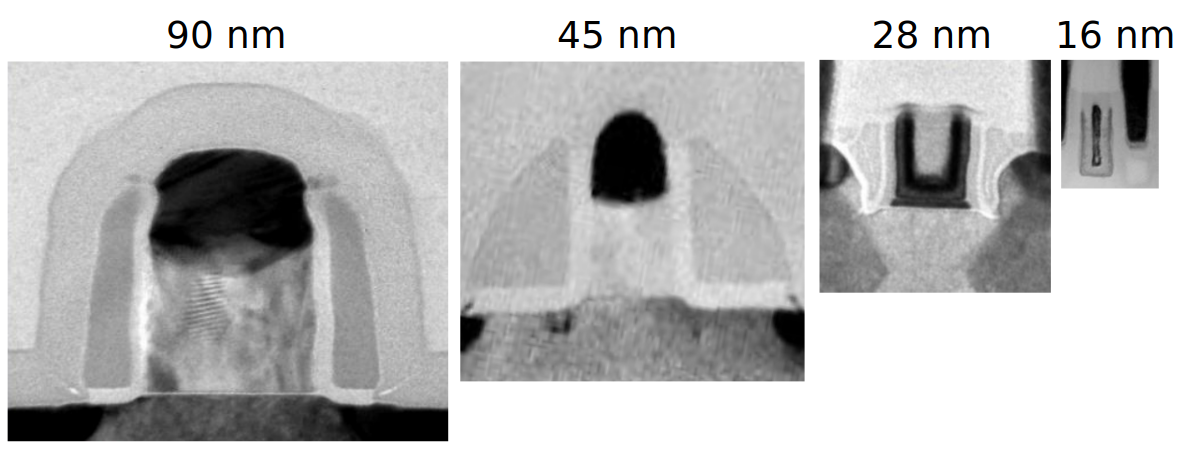
\includegraphics[width=\textwidth]{src/1/figures/technology_evolution.pdf}
  \caption{Recent evolution of NXP's automotive technology nodes \cite{evolution_technologies}}
  \label{fig:nxp-techno-increase}
\end{figure}

% Side effects of size reduction
As a side effect, integrated circuits become more fragile and sensitive.
Maximum tolerated voltage and current levels are smaller.
Above those limits, devices are degraded or destroyed.
The silicon area required for protecting the devices becomes a larger fraction of the complete chip area \cite{evolution_technologies}, and thus of the cost.

% Another trend in automotive - more electronic functions
Nowadays, new major features are developped in the automotive field.
The development of assisted or fully autonomous driving is seeing tremendous progress.
Autonomous vehicles take decisions and perform critical actions such as braking or steering the wheel.
Thoses features are implemented for safety purposes and put very high responsabilities on electronic modules.
Electric cars raise new challenges for safety as well, such as battery management.
Those features require more computing power, more sensing capabilities and more data to exchange.
As a consequence, the amount of \gls{ecu}s and electronic modules in a car is growing quickly.
Communication buses like the \gls{can} \cite{CAN} or \gls{lin} \cite{LIN} are shared by multiple systems and new standards appear for supporting higher bandwidths.
The CAN bus with Flexible Data rate (CAN-FD) is an example of this trend.

% Another trend is reduced power consumptions
Electrical power consumption has largely increased in vehicles.
Solutions are progressively set up to reduce it.
At the integrated circuit level, the main solution so far is to lower supply voltages.
With the most recent technology nodes, it is now common to find supply voltages near 1V.
Noise margins become very small, resulting in circuits far more sensitive to electrical disturbances.

% Harsh environment in the automotive field
The automotive field is also an harsh environment for electronic devices.
Equipements are exposed to a wide range of stresses.
A running engine generates plenty of vibrations and mechanical stress.
A lot of heat and thermal cycling is produced when the engine is on, and a vehicle is exposed to large temperature variations during its lifetime.
Electrical contacts, solder joints and connections suffer from these stresses, and must be designed to withstand them.
Electronic system are also exposed to a wide range of electrical stresses especially in the automotive field.
There are many sources of electrical stresses in a vehicle.
Transient disturbances can be generated natural phenomena, by the vehicle itself or some of its components.
When the engine is turned on for instance, the battery voltage can drop very low because of the amount of current drawn by the ignition.
This voltage drop can affect electronic systems and damage them.
This kind of disturbance is generated by the vehicle itself, but there is another major source of electrical stress coming from a natural phenomenon, called \gls{esd}.

% What is an ESD
An electrostatic discharge is the sudden flow of electricity between two objects of different charge.
It is the result of a local accumulation of electrostatic potential.
When a large enough potential difference is reached, a very rapid and violent discharge occurs.
It is common to record amplitudes in the range of thousands of volts and tens of amperes.
A study by Renault car manufacturer \cite{Renault-esd} estimates that electronic devices are exposed 10000 times to \gls{esd}s during their lifetime.
It has always been considered a very serious threat for electronic systems.

% Architecture systemes automobiles
In terms of architecture, a vehicle is constituted by a multitude of electronic modules, interconnected with cables.
This architecture raises some challenges for guaranting robustness against electrical disturbances.
A car is connected to the earth's ground through the tires, which is equivalent to a thick layer of insulating material.
Interconnected electronic systems need to share a good ground reference for them to communicate and work properly.
This function is assumed by the car's metallic body.
In \gls{dc} and at low frequencies, this reference is quite good because the vehicle's body is a very large chunck of metal with a very low resistance.
Electrostatic discharges are high frequency events, with significant frequency content up to a gigahertz.
In this frequency range, the car's body is not a low value resistor anymore and cables behave as large inductances.
As a result, electronic modules do not share a good reference and can be disturbed and fail to function properly.
For electrostatic discharges and \gls{emc} in general, cables are an important issue.
Inside a car, cables are not shielded and make great antennas that can both receive and emit radiated interferences.
Couplings between cables propagate interferences between interconnect domains.
Overall, the architecture of a vehicle is complex and sensitive to electrical disturbances.

\begin{figure}[!h]
  \centering
  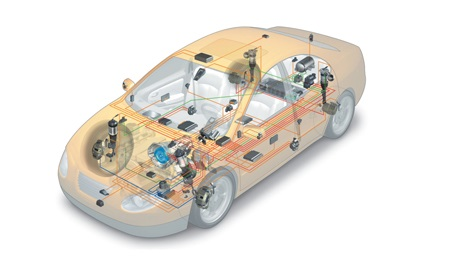
\includegraphics[width=0.7\textwidth]{src/1/figures/systemintegration_01_uv-data.jpg}
  \caption{Architecture of electronic systems in a vehicle \cite{car-architecture}}
  \label{fig:car-architecture}
\end{figure}

% Fiabilite vis a vis des ESD
In summary, the amount of electronic devices is increasing and in the same time they become more sensitive.
Systems are complex to study and analyse, have more responsabilities in regards of our safety, and the surrounding environment is very harsh.
Studying and predicting all kinds of failures is important in order to avoid them early.
In the \gls{esd} field, there are two kinds of failures to consider.
The hardware failure, or hard-failure, is when an electronic device is permanently damaged.
There can be multiple signatures, such as apparition of minor defects, important variation of intrisic properties or complete destruction (see Fig. \ref{fig:esd-failures}).
Semiconductor devices are particularly sensitive to electrostatic discharges \cite{impactESDsemiconductors} and require specific protection.
Recently, a new class of failures is being studied, motivated by new requirements for operating safety.
Soft-failure, or functional failure, is when an electronic device fails temporarily to perform its function, because of an electrical disturbance.
In this scenario, different levels of severity can be identified depending on the impact of the failure on the rest of the system.
In the best case, a module is momentarily disturbed by a discharge but recovers immediately without noticeable impact.
In a more severe scenario, some minor functionnalities such as entertainment systems are frozen, requiring an user intervention to recover, in the form of restarting the vehicle for instance.
The same kind of issue with airbags or assisted braking would be considered a lot more severe, because user safety can no longer be guaranteed.
Functionnal failures raise new kind of challenges for the analysis, and in particular with the scale factor.
A functionnal failure may happen because a few transistors inside a chip were disturbed, but the consequences can be visible much higher in the hierarchy and at the scale of an entire vehicle.
In regard of those challenges, new analysis and predictions methods are required against soft-failures caused by electrostatic discharges.

\begin{figure}[!h]
  \centering
  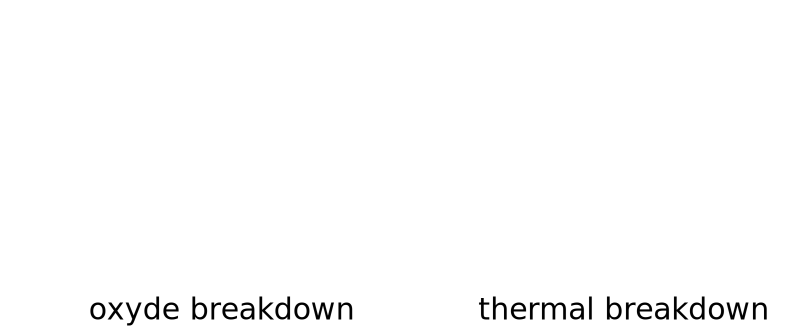
\includegraphics[width=\textwidth]{src/1/figures/esd_failures.pdf}
  \caption{Different kinds of ESD-induced failures}
  \label{fig:esd-failures}
\end{figure}

%TODO: Explain the cost of fixing an issue early vs lately ?

% Comment predire ces defaillances fonctionnelles
First research on the topic was published by F. Caignet and N. Lacrampe in 2007 \cite{}.
After a few years, the industry widely acknowledged the problem, reinforced by the current automotive trends.
A large amount of research at the system level was published in EOS/ESD symposia 2012 \cite{} and 2013 \cite{}.
The draft standard IEC 62433-6 aims to provide a base framework for soft-failures analysis and prediction.
So far, the litterature is focused on system-level analysis.
There is currently no real work at the component level or studies performed inside the design of an integrated circuit.
This PhD explored the topic and tries to provide some new leads for future research.

% Conception methods
Beyond studying failures inside integrated circuits, it is important to keep in mind how chips are designed and developped.
This is important to propose solutions that are actually implementable.
This entire process from the specification to the manufacturing of a product is called the design flow.
During this process, there are many teams and people involved.
Modeling team creates electrical model of technology components.
Design team assembles component together to create integrated functions that conform to the specification.
Layout team translates the symbolic view of electrical netlists into the series of masks and layers required by manufacturing.
The laboratory tests manufactured parts and runs investigations in case of failures.
The \gls{esd} and \gls{emc} team has the particularity to interact will all teams because issues and solutions can be found in any step of the design flow.
Overall, the integrated circuits are designed hierarchically and the flow is a bottom-up process.
Fundamental bricks are assembled together in rising complexity to create the required functions.
The main source of delay in this process is the long delay for the feedback due to the manufacturing.
Designs are put on silicon but the parts are tested only after manufacturing, which can occur several months later.
To gain time to market and be competitive, it is essential to reduce to a bare minimum the amount of design-manufacturing-testing cycles.
This is why any simulation tool able to predict early any kind of failure (and functionnal failures among them) is very valuable for silicon design companies.

\begin{figure}[!h]
  \centering
  \includegraphics[width=\textwidth]{src/1/figures/overview_flow.pdf}
  \caption{Highly simplified integrated circuit design flow - specification, symbolic view, layout, silicon}
  \label{fig:ic-design-flow}
\end{figure}

% Presentation des chapitres
%
Chapter \ref{chap:1} details how electrostatic discharge physically appear, how to reproduce them in laboratory conditions and summarizes recent litterature.
This preliminary work highlights how functional failures appear and how they impact electronic devices.
It is demonstrated that so far integrated circuits are studied as black-box electrical objects.
Stresses are injected on external inputs while external outputs are monitored for failures.
The amount of silicon-level studies and research remains small.

%
Chapter \ref{chap:2} presents a modeling method for simulating \gls{esd} waveforms up to the integrated circuit inputs.
The first challenge for understanding soft-failures at silicon-level is to determine what fraction of an incoming \gls{esd} actually reaches the integrated circuit.
Between the injection point of a stress and the disturbed circuit, many devices are be connected such as cables, discrete devices, etc.
Each element interacts with the discharge, absorbs a part of its current or changes the waveform.
A model library of common electrical elements found in \gls{esd} testing environment has been constructed and is detailed.

%
A case of soft-failure in an integrated circuit is explained in chapter \ref{chap:3}.
In a first phase, measurement data is obtained at the board level and the failure is explained.
Simulations are run to understand how failures appear, and more specifically how a short electrical event can disturb an integrated circuit for a long period of time.
In a second phase, the integrated function is placed onto a custom testchip.
Specific on-silicon structures were designed to gather measurement data on electrical nets that are not physically accessible.
All these measurements are performed for the purpose of estimating the accuracy of integrated circuit \gls{esd} simulations.
There are two main potential sources of error that are checked.
Silicon technology device models are not designed to function for extremely fast transient transient disturbances.
Also, standard simulations do not take parasitic devices into account, such as metal track resistances and parasitic couplings.
Measurement data is confronted to simulations in order to verify the validity of models.
Analysis of the failure led to the development of a testchip, to put on silicon the same failing function but with a more convenient environment for measurements and investigation.

%
When issues are discovered late in the testing lab, analysis is performed manually, by trial and error, searching inside the design why the function is failing.
It is a complex and time-consuming process.
The core research of this work focuses proposing new analysis methods and tools for electrical simulations.
It is detailled in chapter \ref{sec:methods-operating-esd-analysis}.

%
Finally, a new test generator was developed to overcome some issues found when debugging silicon-level failures caused by system level \gls{esd} testers.
The principle of operation and architecture of the generator is described in chapter \ref{sec:tlp-hmm}.
The conclusion summarizes the work achieved during the PhD, highlights the most notable discoveries, and identifies follow-up work and research topics that could be worth pursuing.
Some part of the research work also focused towards \gls{esd} testers.
System-level \gls{esd} guns \cite{iec61000-4-2, iso10605} constitute a major testing and qualification tool, but bring too much complexity during silicon-level investigation.
To overcome this issue, a new stress generator based on a \gls{tlp} is proposed in chapter \ref{sec:tlp-hmm}.
It produces the same compliant waveform than those standards, but with some interesting advantages.
It is not a drop-in replacement but can be interesting as an investigation tool.

%
Final conclusions and potential following work are detailed in chapter \ref{sec:final-conclusion}.

% Chapter files listing
\chapter{Review of ESD testing and functional analysis}
\label{chap:1}

\section{Electrostatic discharges in the automotive field}
\subsection{General concept}

% What is an ESD
\gls{esd} is the sudden flow of electricity between two differently-charged objects.
It is the result of the accumulation of electrostatic potential through tribocharging or electrostatic induction.
The discharge itself is caused either by contact, electrical short or dielectric breakdown.
Through static electricity buildup, thousands of volts can be accumulated locally, until a discharge happens.

% What are its key properties
\gls{esd} events have very short timespan, usually in the range of a few hundred nanoseconds.
Although very short, it is frequently observes flowing currents in the range of tens of amperes.
As a result, the overall discharge energy is small, but the power is extremely high.

% Impact
Such harsh events are very harmful for electronic systems and integrated circuits.
Today, there is not a single device in the field that is not protected against electrostatic discharges.
Due to the very short, fast, and random nature of \gls{esd} events, it remains very challenging to perfectly protect an electronic system against them.

\subsection{Generation mechanism in the automotive field}

% Harsh automotive field is harsh
From a general perspective, the automotive field is a harsh environment for electronic devices.
Equipements are exposed to a wide range of mechanical, electrical and thermal stresses.
A running engine generates plenty of vibrations, that can wear out electrical contacts, solder joints and connections.
It also generates heat, and a car can be exposed to large temperature variations during its lifetime.
Integrated circuits must be designed with those constraints in mind.

%TODO: References
% ... Especially for ESD
The automotive field has also the harshest requirements for \gls{esd}.
When a car is moving on the road, two different mechanisms generate static electricity accumulation.
Electronic devices inside a car are therefore constantly exposed to electrostatic discharges.

% Detail the first mechanism
When the car is moving on the road, the friction between the rubber wheels and the road generates tribo-electricity.
Basically, charges are stripped-off between the wheels and the road, leading to the accumulation of charges on the vehicle.

% Detail the second mechanism
Similarly, the friction between the car's body and the air flowing through it generates charge accumulation on the vehicle.

% How does the discharge happens
When electrostatic potentials become large enough, dielectric barrier breaks down and and a discharge happens.
It propagates through the car's body, wiring and electronic equipments.

\subsection{Impact of ESD on electronic devices}

%TODO: Pictures
% Electronic devices are exposed to ESD, in factories first
As detailed in the introduction, electrostatic discharges constitute a large threat for electronic devices.
Failures can occur during manufacturing and or normal operation.
The manipulation of parts by manufacturing machines involves repeated contact and separation.
Ultimately, triboelectrification and discharges happen and devices can get destroyed.
Several standards exist to guarantee that devices can survive this manufacturing step.

% HBM
The Human Body Model (HBM) reproduces the discharge of a human body into a device.
It is standardized in Method 3015.9 of MIL-STD-883 \cite{MIL-STD-883} and JEDEC JS-001-2014 \cite{jedec-001}.
The charged human body is modeled by a 100 pF capacitor and a discharge resistor of 1.5 k\textOmega{}.
Charging voltages reach a maximum of 8kV, although nowadays customers tend to ask for less than that.

% CDM
The Charged Device Model (CDM) is a field-induced ESD test.
The component under test is placed between two charging plates that generate an electric field.
At some point, a grounded pin is brought near any of the pins of the component, forcing the charges to evacuate suddenly.
This test is standardized in \cite{jedec-002}.

% MM
The Machine Model (MM) used to be another ESD testing specification that is now considered deprecated.
The JEDEC committee recommended discontinuing use of this standard \cite{discontinued-mm}, because it is the result of a misunderstanding of real-world events in manufacturing environments.
It does not help improving the reliability of devices against electrostatic discharges.

% HMM ?

%
Over the years, manufacturing processes and standards have improved, reducing the requirements of discharge levels to sustain.
In parallel, the factory environment has been studied extensively to identify actual levels devices are exposed to.
Machine Model deprecation is the perfect illustration of increased community knowledge and experience.
Those efforts aim to reduce the pressure on semiconductor manufacturers that are facing growing challenges to protect devices, because of the shrink of technologies and robustness.

% Electronic devices are exposed to ESD in the field
After manufacturing, failures can happen with the device in the field and exposed to its operating environment.
Manipulation by electrically-charged humans is a major source of danger for commercial products like cellphones and cameras.
The automotive environment is even harsher, with vehicles being a major source of electrostatic discharges.

% Main impact is hard-failure
The electrical destruction of a device is called a hard-failure.
A hard-failure corresponds to changes in the material structure or properties of a device to the point where it no longer fullfills at least part of its specification.
\gls{esd} induce those failures because of the extremely large current densities, high voltages, and power levels involved.
Different kinds of failure signatures can be observed.
Pictures of destroyed devices, obtained with an electronic microscope, are provided in Fig. \ref{fig:silicon-level-failures}.
%TODO: Comment

\begin{figure}[!h]
  \centering
  \includegraphics[width=0.3\textwidth]{src/1/figures/example_silicon_failures.pdf}
  \caption{Example of ESD induced failures at silicon-level}
  \label{fig:silicon-level-failures}
\end{figure}


% Oxyde breakdown
%TODO: Etoffer avec these monnereau
%TODO: Values
A first kind of common failure for integrated devices is the oxyde breakdown.
Oxyde breakdown happens when an insulating material is exposed to a larger electric field than it can tolerate.
During an \gls{esd}, large voltage variations in a short amount of time result in very large electric fields superior to 1kV/m ?
For reference, thunder and lightning events have electrical fields in the same order of magnitude.
Oxyde breakdown is usually discovered in the insulator constituting the gate of a \gls{mos} transistor.
As technologies shrink, so does transistor gate oxyde thickness (TODO: Citer presentation).
A thinner gate oxyde can tolerate less electrical field ?
After the failure, the gate that is normally insulated from the rest of the device leaks significant amount of current.
The transistor can no longer operate and is considered destroyed.

% Thermal breakdown
Thermal breakdown is another kind of ESD induced failure.
It is the result of an elevation of temperature inside the silicon, above its melting point.
It is caused for long discharges that can induce significant and very localized device heating.
It results in a significant increase of leakage current or apparition of short-circuits.

% Metal melt
Finally, metal melt is the last kind of failures observed after a discharge.
Inside an integrated circuit, metal tracks are rather resistive because of their form factor.
Resistivity sits in the range of 10m\textOmega{}/$\Box$ to 100m\textOmega/$\Box$.
When large currents are flowing, metal tracks and vias dissipate power and heat up.
The elevation of temperature, if large enough, can melt the metal track and turn it into an open-circuit.

% Hard-failure is one thing, soft-fail another
Integrated circuits are studied and protected against hard-failure since a few decades.
Despite this experience of the \gls{esd} community, it remains challenging to perfectly protect an electronic system against hard-failures.
Nowadays, a new class of failures appears.
Instead of studying permanent failures, devices are studied for temporary failures affecting their functionality.
These are called soft-failures or functional failures.
\gls{esd} can cause them to happen, with diverse consequences.
In less severe situations, functionnality of a chip is disturbed just for the duration of the ESD and recovers immediately without noticeable consequence.
The failure remains located inside the integrated circuit and does not impact the application above.
Sometimes, the discharge is harmful enough to cause a circuit to restart because the \gls{esd} disturbed some critial nets or parameters.
This is common when supply voltages go out of specification for instance.
Startups or power-on reset functions understands overvoltage or undervoltage as the signal for a regular power-up sequence.
The device can also perform restarts to try a recovery because proper operations cannot be guaranteed, due to unexpected values on some nets.
Most microcontrollers for instance monitor supply voltages of digital gates.
If the voltage is too low, the noise margins of the gates cannot be guaranteed and proper operations either.
At this point, the microcontroller restarts to try to recover.
Restarts are slow processes compared to the operation of a chip.
For critical applications, this delay is highly unwanted because it impacts human safety.
The availability of the chip that triggers airbags in a car is vital for instance.
In a more severe scenario, the system gets completely frozen or stuck into an unwanted state because of the \gls{esd}.
The only way to recover normal operation requires a user-intervention.
User intervention can take the form of turning the key to shut down and restart the vehicle's engine.
Finally, hard-failure can be seen as the next step immediately after the most severe soft-failure.
The device is in a non-recoverable state and must be replaced.
Hard-failures are not considered for functional robustness analysis.

% What is the challenge
In this context, soft-failures represent a risk just as important as hardware failures.
To limit risks and costs inherents to upgrading a device after it was deployed in the field, these failures must be taken care of as early as possible.
Ideally, the robustness of an electronic product should be studied, characterized or simulated during its design phase.
The research conducted and presented in this document aims to develop new tools and techniques for studying and predicting functional failures.

% Protection of integrated circuits against hard-failure is done with ESD protections
To protect sensitive electronics against discharges, several options are available.
The most common solution, presented in the next section, is the \gls{esd} protection.

\subsection{ESD protection}

% Principle of operation
\gls{esd} protections deviate discharge current before it reaches sensitive circuitry and clamp input voltages to avoid crossing the maximum tolerated levels.
Fig. \ref{fig:esd-protection-strategy} gives a simple example of \gls{esd} protection strategy.
Current is routed into the ground before reaching the core-circuitry.
Protections have very low on-resistance, usually in the order of a few ohms.
Even with a few amperes of current, voltage remains low.
\gls{esd} protections can absorb significant amounts of current for very short periods of time, but they are not designed to sustain DC currents.

\begin{figure}[!h]
  \centering
  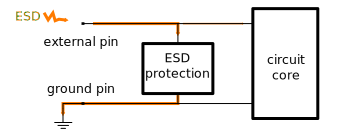
\includegraphics[width=0.3\textwidth]{src/1/figures/esd_protection_strategy.pdf}
  \caption{Classic ESD protection strategy}
  \label{fig:esd-protection-strategy}
\end{figure}

% Types of protection
Inside an electronic circuit, ESD protections are usually found in two different locations.
On-chip protections are integrated directly into silicon.
External protections are discrete devices connected to the input of an \gls{ic}.
Historically, on-chip protections were designed to protect integrated circuits against stresses generated during manufacturing.
They were not aimed to protect against system-level discharges, i.e. discharges happening in the field during the normal product life.
This task was fullfilled by external protections, such as TVS, diodes, capacitors, filters, etc.
Over the years, design techniques and simulations tools improved, and more robust integrated protections could be designed.
On the other hand, equipment manufacturer were always looking for means of reducing the \gls{bom} or the cost of electronic systems.
This lead to a shift of responsabilities for protecting against system-level stresses toward on-chip \gls{esd} protections.
The shrink of integrated technologies makes this tasks ever more challenging.
External protections are still very relevant, where an integration solution would occupy too much silicon area, or when very harsh requirements are demanded.

\begin{figure}[!h]
  \centering
  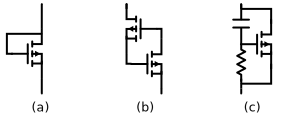
\includegraphics[width=0.3\textwidth]{src/1/figures/architecture_esd_protections.pdf}
  \caption{common ESD protections architectures - (a) Diode (b) Thyristor (c) RC-triggered MOS (d) ?}
  \label{fig:architecture-esd-protection}
\end{figure}

% Implementation and common architectures
ESD protections can be designed in various ways (see Fig. \ref{fig:architecture-esd-protection}).
Diodes are commonly found.
They are not necessarily the more compact solution on silicon, but they can protect properly sensitive circuitry.
Thyristor architectures are frequently used too.
Below triggering voltage, the structure is completely off and disconnected.
Above it, the thyristor switches on, absorbs current, and stays on until the discharges is over and the current returns to a small value.
Thyristors have typical snapback characteristics as shown in Fig. \ref{fig:iv-curve-esd-protection}.
RC-triggered \gls{mos} are frequently found for protecting low-voltage \gls{io} of \gls{cmos} circuits.
Basically, it is a power transistor activated during the discharge by a resistor-capacitor network.
The capacitor is most of the time the parasitic gate capacitance to ground (TODO: check).
During a transient event, the capacitor acts as a short-circuit, rising the gate potential.
The \gls{mos} switches on and absorbs current, deviating it into the ground.

%TODO: Put leakage curve
\begin{figure}[!h]
  \centering
  \includegraphics[width=0.3\textwidth]{src/1/figures/iv_curves_esd_protections.pdf}
  \caption{I(V) curves of typical ESD protections with snapback and no-snapback}
  \label{fig:iv-curve-esd-protection}
\end{figure}

% Comment IV curve
A few key values are important for describing a protection.
V\textsubscript{t1} refers to the triggering voltage of the protection.
I\textsubscript{t1} (snapback devices only ?) corresponds the current absorbed by the protection immediately after triggering.
V\textsubscript{t2} and I\textsubscript{t2} describe the coordinates where the protection is destroyed.
A sudden increase of the leakage current (Fig. \ref{fig:iv-curve-esd-protection}) is a good indicator of a damaged protection.
Leakage current is extracted with a DC source, with a compliancy value set very low, usually below the milli-ampere of current.

%TODO: Talk about protection strategies, centralized clamp vs distributed. RC-mos + boost rail to trigger all protections, etc.

% Requirements
To design a efficient \gls{esd} protection, several constraints and requirements must be fullfilled.
In the absence of a discharge, protections must be transparent to the rest of the device.
The protection must trigger above the operating voltage of the circuitry.
If an input operates between 0V and 5V, and the protection switches on at 4V, it will trigger during normal operation and be immediately destroyed.
On the other hand, protections must trigger below the maximum voltage tolerated by the silicon technology.
If the integrated technology accepts voltages below 50V, and the protection triggers at 60V, the circuit will be destroyed.
Therefore, they are designed to operate between those two boundaries which delimit the \gls{soa} (see Fig. \ref{fig:soa-esd-protection}).
For demanding applications, protections must trigger at a given voltage accurately, independently of manufacturing process, layers mismatches and temperature variation.
This reduces the \gls{soa} substantially and makes the design more challenging.

\begin{figure}[!h]
  \centering
  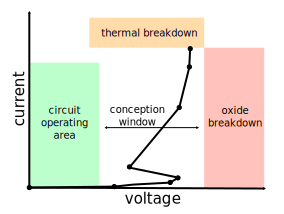
\includegraphics[width=0.3\textwidth]{src/1/figures/esd_protection_soa.pdf}
  \caption{Safe-Operating Area of an ESD protection}
  \label{fig:soa-esd-protection}
\end{figure}

% Tools
To design and validate protections, tools like Centaurus TCAD \cite{TODO} are employed to simulate semiconductor physics.
Afterwards, an electrical model is constructed, to verify that the protection and the circuit cooperate as expected.
Simulation is ran in a \gls{spice} environment, such as Cadence Virtuoso \cite{TODO} or Mentor Graphics SimVision \cite{TODO}.
Modelling of \gls{esd} protections for \gls{spice} simulations is presented later in chapter \ref{esd-protection-modelling}.

\section{State of the art in ESD testing}

To ensure proper operation once in the field, hardware is tested against \gls{esd} using different test methods and standards.
The goal for each method is to reproduce a particular \gls{esd} waveform in lab conditions.
In this chapter, we will introduce most relevant \gls{esd} generators, which will be useful later on for modeling them accurately.

In ESD testing, distinction is often made between so-called system-level level tests and \gls{ic} level tests.
The first kind reproduces \gls{esd} events that a system deployed in the field may encounter during its lifetime, while the latter is targeting \gls{esd} events
happening during \gls{ic} manufactoring.

System-level tests involve higher voltage and current amplitudes, and are more harmful for electronic devices than \gls{ic} level tests.
EXTERNAL DEVICES FOR PROTECTING ?
ICs now have to sustain SYSTEM level tests

\subsection{Transmission Line Pulsing (TLP)}

\gls{tlp} generators generate a fast rectangular pulse \ref{tlp_concept}.
The pulse is produced by the discharge of a coaxial cable.
The cable is charged by a high-voltage power supply then discharged into a load by switching a relay.

\begin{figure}[h]
  \centering
  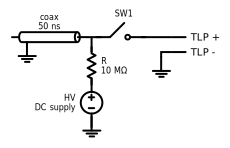
\includegraphics{src/1/figures/tlp_concept.pdf}
  \caption{Minimal example of a \gls{tlp} system}
  \label{tlp_concept}
\end{figure}

The charge is performed through a high value resistor to keep the current small and avoid generating oscillations on the cable.

TLP systems constitute very well-controlled test generators, because the pulse is generated inside a shielded and isolated environment.
Characteristic impedance can be controlled up to the load.
Those features allow for extremely clean and repeatable pulse waveforms.
Main characteristics of a TLP waveform are given in figure \ref{tlp_pulse}

\begin{figure}[h]
  \centering
  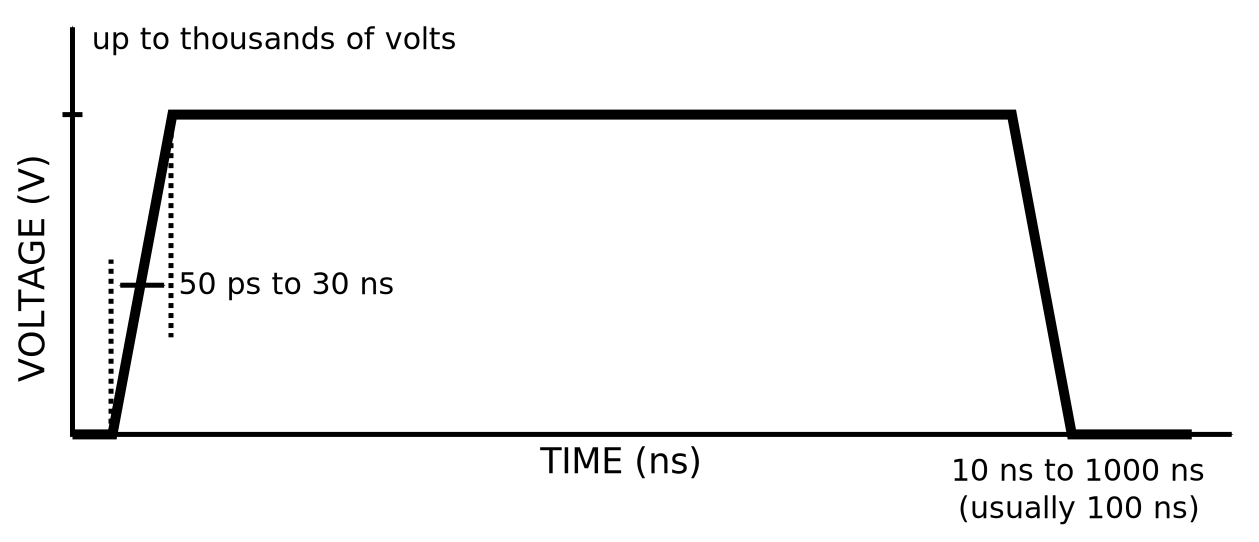
\includegraphics[width=\textwidth]{src/1/figures/tlp_pulse.pdf}
  \caption{Main characteristics of a \gls{tlp} pulse on a resistive load}
  \label{tlp_pulse}
\end{figure}

Using time-domain reflectometry, it is possible to reconstitute the current and voltage waveforms inside the load,
from measured current and voltage inside the \gls{tlp} \cite{TLP}.
The superposition of the incident and reflected pulses during the discharge show that the voltage and current
measured inside the generator are direct image of the ones accross and through the load.

\gls{tlp} are extensively used for characterizing the response of ESD protections \cite{TLPforESDProtectionCz}
or testing the response of systems and devices against a clean and well repeatable pulse \cite{TLPthroubleshooting, LacrampeTransientImmunity}.

\subsection{ESD Gun (IEC 61000-4-2 / ISO 10605)}
The system-level ESD Gun aims at reproducing the discharge of a human body through an electronic device.
This test is used extensively for the qualification of products.

\begin{figure}[h]
  \centering
  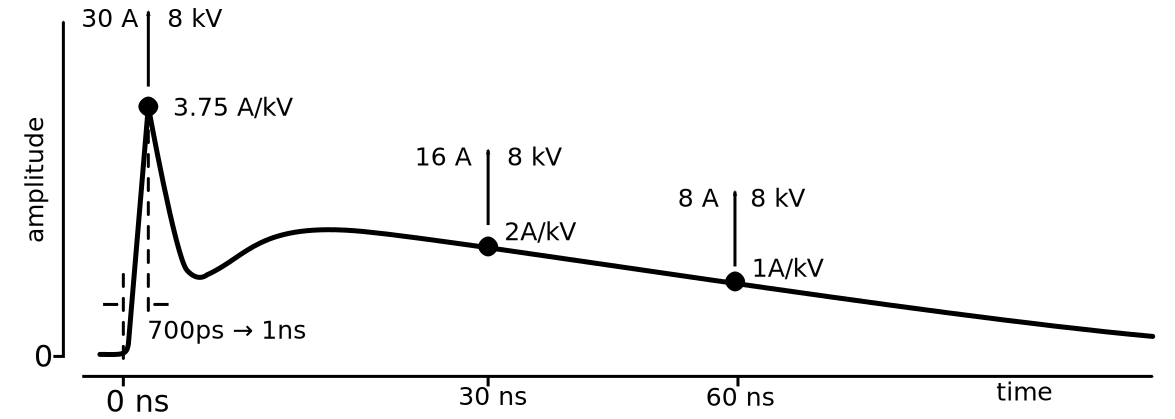
\includegraphics[width=\textwidth]{src/1/figures/iec61000-4-2_waveform.pdf}
  \caption{Main characteristics of an IEC 61000-4-2 pulse on a 2&\X\Omega resistive load}
  \label{iec_pulse}
\end{figure}

The generation of the ESD pulse is done by an resistor-capacitor discharge network, however, the RC network alone does not suffice to reproduce the waveform given \ref{iec_pulse}.
Parasitic devices play an important part in shaping the waveform.

Two standards define the construction and waveform requirements for this ESD generator, but with different fields of application.

IEC 61000-4-2\cite{iec61000-4-2} standard targets consumer electronics, while ISO 10605\cite{iso10605} standard is intented for automotive equipment.
The latter defines additional pulse waveforms to cover a wider range of ESD events (See fig \ref{iso_pulse}).

\begin{figure}[h]
  \centering
  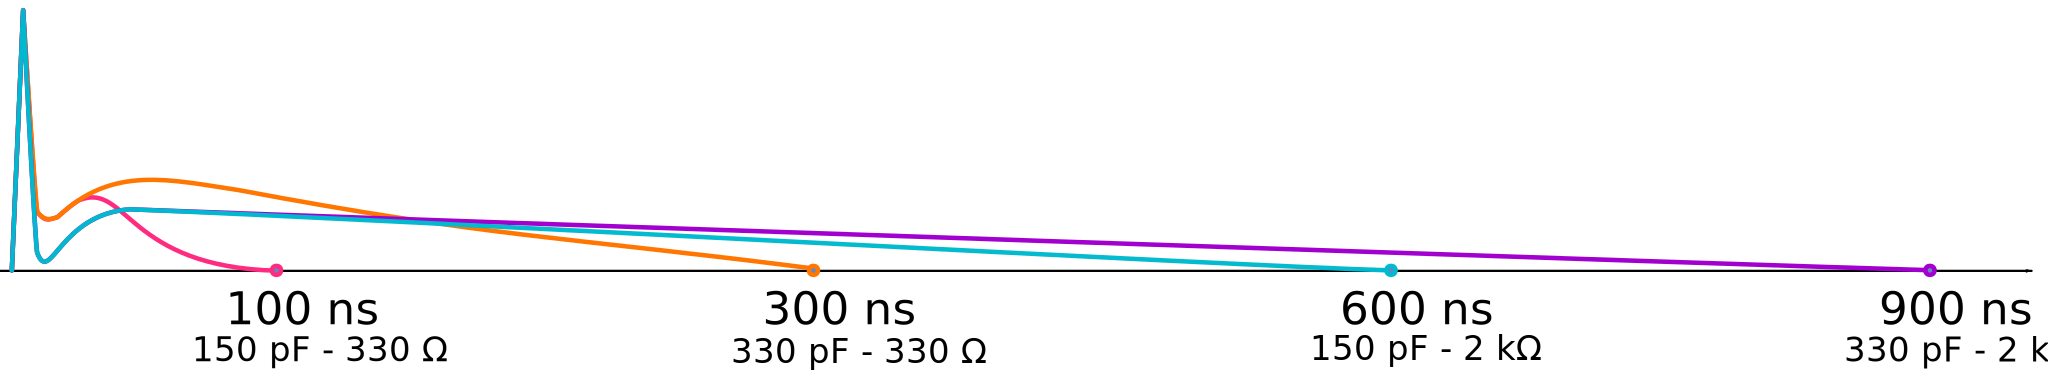
\includegraphics[width=\textwidth]{src/1/figures/iso10605_waveform.pdf}
  \caption{All waveforms defined in ISO 10605 standard on a 2&\X\Omega resistive load}
  \label{iso_pulse}
\end{figure}


\subsection{ISO 7637-2}
ISO 7637-2\cite{iso7637-2} is an automotive standard for testing immunity of electronic devices against transient electrical disturbances.
It is mostly targeting disturbances applied on supply lines.
This standard gathers many different pulses. Pulse 2A and 3B are in the ESD timescale.

Pulse 2A simulates the sudden disconnection of a load placed in parallel with the \ref{dut}.

SCHEMA

The parasitic inductance of the wiring harness is opposing to this interruption of current.
Instead of flowing through the load, this extra transient current is reported on the \ref{dut} which can be damaged or disturbed in the process.

The characteristics of pulse 2A are given in fig. \ref{...?}

PULSE 2A waveform

On the other side, pulse 3B simulates the result of a switching process with a wiring harness.
The waveform is similar to pulse 2a, but with a shorter duration and risetime and higher amplitude.

PULSE 3A waveform

\subsection{Burst test (IEC 61000-4-4)}

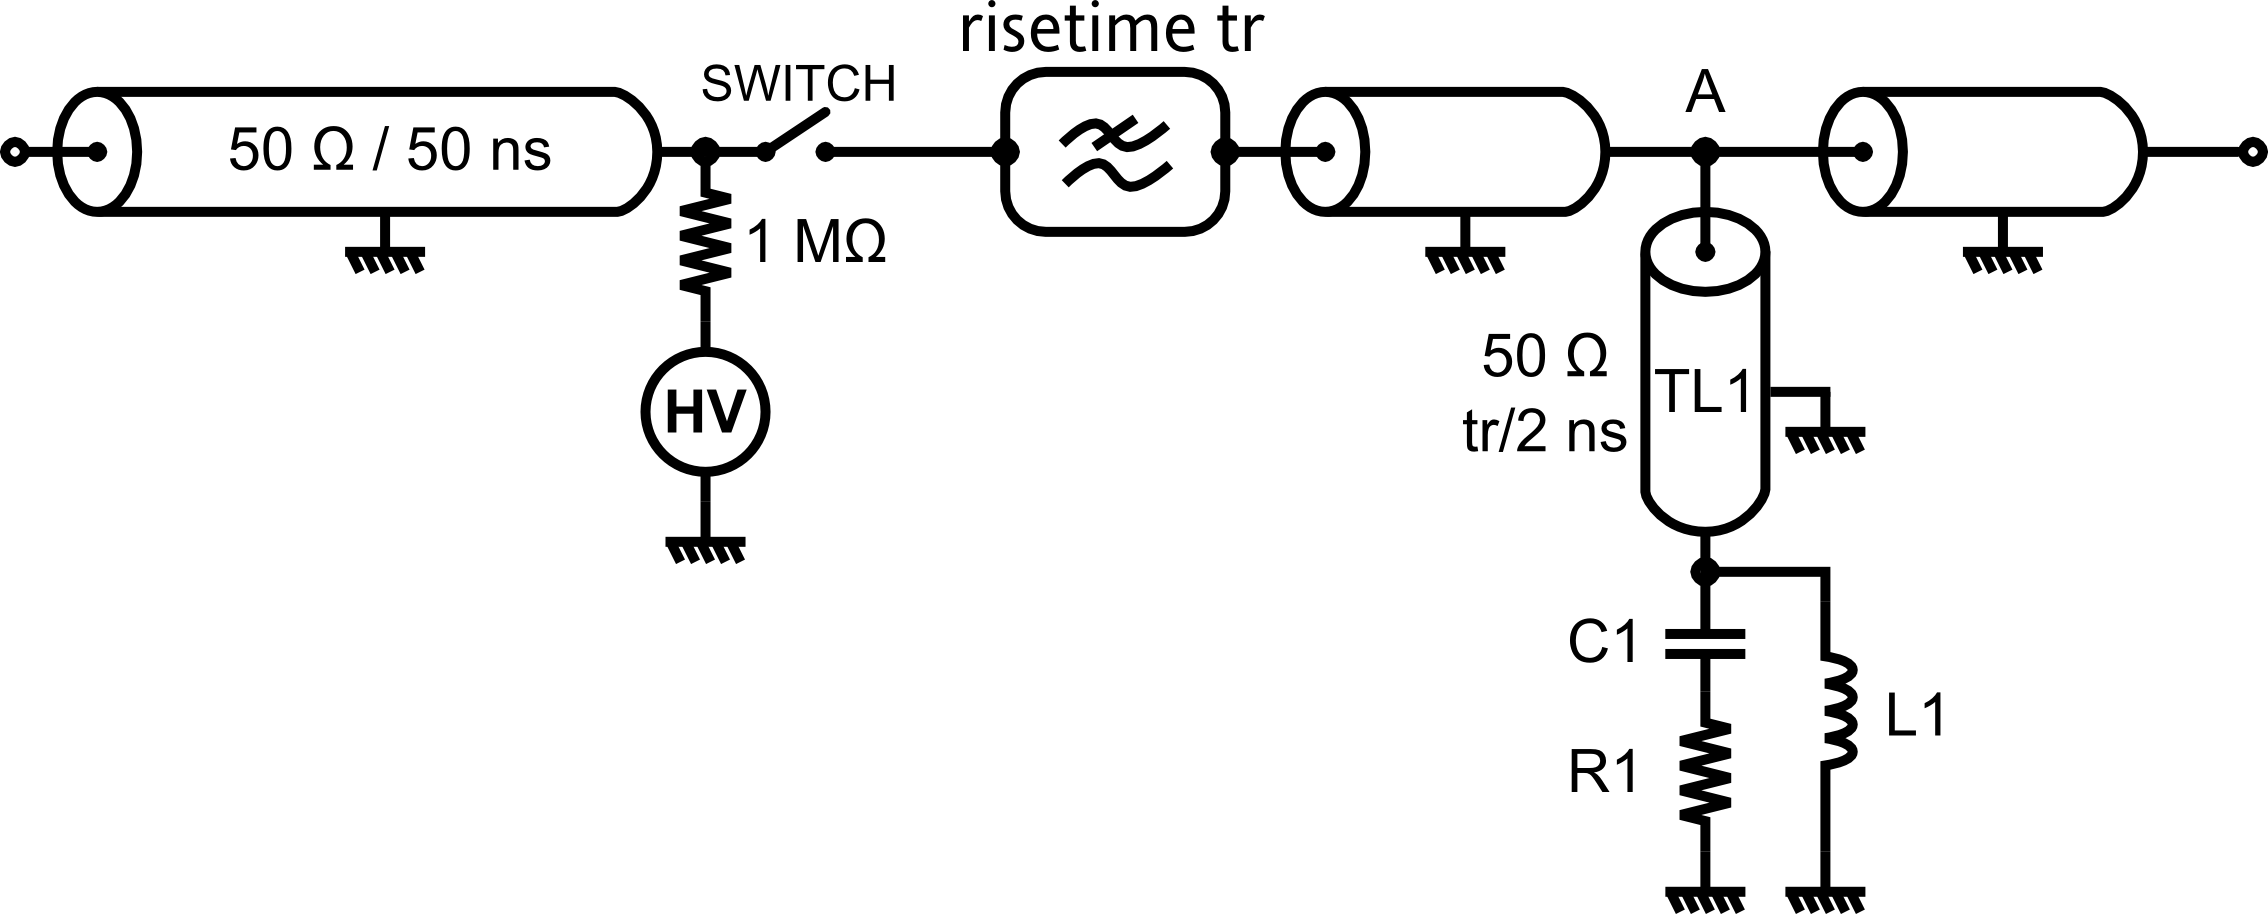
\includegraphics[width=\textwidth,height=\textheight,keepaspectratio]{src/2/figures/tlp_iec.png}

\section{Review of soft-failure silicon-level investigation}

In previous sections, major \gls{esd} standards used in laboratories were presented.
The impact of electrostatic discharges on electronic devices has been detailed, highlighting two classes of failures.
Hard-failures are well known and multiple protection strategies exists, from external devices and ESD protections, to distributed protection architectures and much more.
Soft-failures are the kind of issue caused by electrical fast transients.
When discharges propagate inside electronic equipments and reach integrated circuits, they can cause them to malfunction.
For multiple reasons described in previous sections, it is essential to detect early functional weaknesses.
This section is a review the literature of the current state of the art on \gls{esd} induced soft-failure analysis.
Study cases, observation methods and modeling approaches are presented.

\subsection{Case studies}

% Case 2 - CESAME IC - paper Vrignon + Ben dhia
N. Lacrampe presents a functional failure case in \cite{LacrampeTransientImmunity}.
Very-fast \gls{tlp} is injected on an \SI{0.18}{\micro\metre} CMOS technology (\SI{1.8}{\volt} supply voltage) testchip.
The chip contains 6 instances on the same logic core, differing only by their power-rails architecture.
The injection on power rails is performed using a \gls{dc} block \SI{1}{\nano\farad} capacitor, similarly to the \gls{dpi} standard \cite{iec62132-4}.
% What is the failure signature
An output signal of the logic core is monitored.
The susceptibility criteria is the amplitude crossing a \SI{20}{\percent} threshold from the established logic level.
Above this threshold, the core is supposed to no longer work reliably.
It is proven that modeling the output buffer of the core logic is enough for reproducing with less than 20\% error the waveform on the output.
It is less accurate than a full-netlist simulation, but faster to simulate.
VHDL-AMS and \gls{spice} modeling are performed in this analysis.

% Case 3 - failures on an SDRAM
In \cite{SDRAMCase}, soft-failures are studied on a SDRAM memory in operation.
The injection setup consists of a modified compact \gls{tem} cell \ref{fig:modified-tem-cell} with a reduced septum height.
Reduced dimensions result in increased field strengths, to reach levels normally produced by an \gls{esd} gun.
The discharge waveform, injected inside the cell, is generated by a filtered \gls{tlp} and is similar in shape to IEC 61000-4-2 \cite{iec61000-4-2}.
The SDRAM chip is mounted on a board.
Data is written and read on the memory by a \gls{fpga}.
Differences between incoming and outgoing data signifies a functional failure of the memory.
Only the memory is exposed to the disturbance, the rest of the board's devices are located outside of the \gls{tem} cell, on the other side of the board.
The main defect of this method is to only provide a global failure level.
It does not allow to identify which particular net or pin is the most sensitive to disturbances.

\begin{figure}[!h]
  \centering
  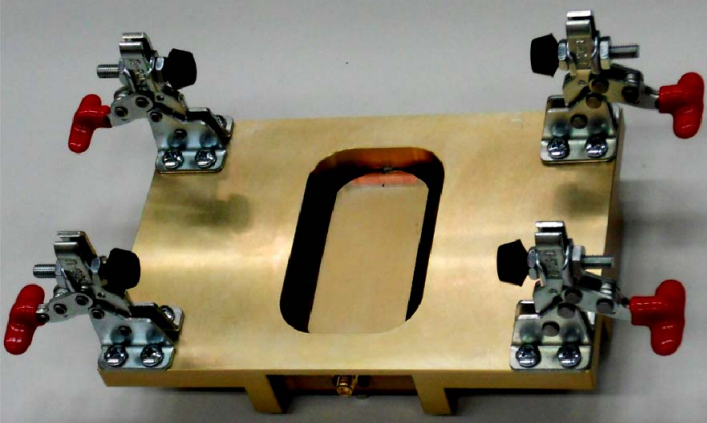
\includegraphics[width=0.6\textwidth]{src/1/figures/modified_tem_cell.png}
  \caption{Modified TEM cell from \cite{SDRAMCase}}
  \label{fig:modified-tem-cell}
\end{figure}

B. Orr reports in \cite{softFailSubsystem} errors caused by electrostatic discharges on two different camera communication buses.
Events of different severities are observed, depending on the discharge parameters.
It is attempted to determine whether the sensor or the application processor is causing the error.
The magnetic emission map is recorded with a near-field magnetic scanner to try to observe local variations in the emission spectrum because of the degradation of functionality.
It was envisioned that soft-failure can induce significant variations in the emission spectrum of a disturbed component, and thus those variations could help localize them.
In this particular case, the root cause of failures could not be determined.

An LCD display is studied in \cite{softFailLCD}.
The device is tested with an IEC 61000-4-2 \cite{iec61000-4-2} generator, and non-destructive problems are observed due to the discharge.
Electromagnetic disturbances cause stripes to appear on the display, optical parameters changes and black-lighting malfunctions.
System-level testing waveforms were found too complex for identifying the root cause.
A near-field injection is performed to identify which trace of the LCD's flex connector claims the lowest immunity.
The lack of resolution of the near-field probe caused multiple traces to be disturbed at once, preventing this second approach to work.
Finally, the individual track stressing was repeated with a capacitively-coupled \gls{tlp} on each individual metal track.
However, results were once more inconclusive and no metal trace could categorically be identified as more sensitive than the others.
The conclusion for this paper is that silicon level soft-error models are required for standard investigation.

An investigation method is presented in \cite{softFailMobile} to search for discharge propagation paths responsible for soft-failures on a mobile phone.
The IEC 61000-4-2 standard is chosen as testing waveform.
Metallic parts are assumed to be the main propagation paths.
To confirm this hypothesis, time-domain electromagnetic field 3D simulations of almost the entire phone are ran (see Fig. \ref{fig:mobile-phone-3d-em})
After the failure location was determined, RC-networks are used as countermeasures to protect physical inputs and outputs, like buttons, LCD inputs and connectors.

\begin{figure}[!h]
  \centering
  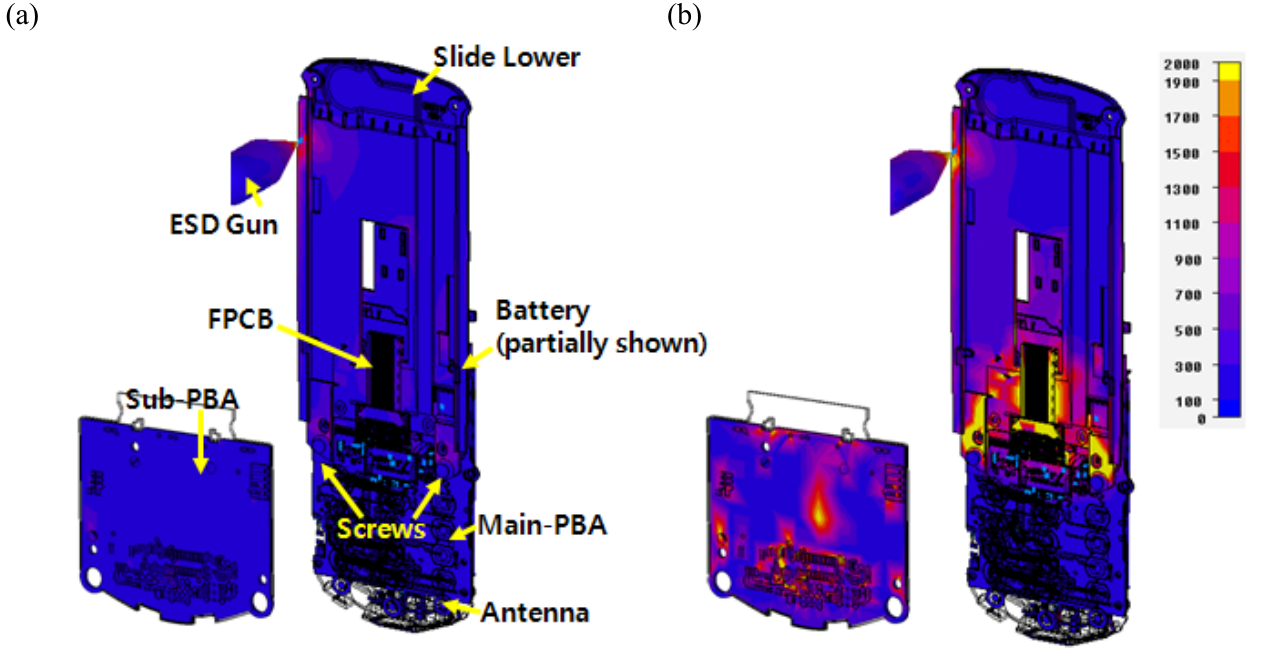
\includegraphics[width=0.8\textwidth]{src/1/figures/current_distribution_mobile.png}
  \caption{ESD Current Distribution on Mobile Phone and Backside sub-battery pack at (a) \SI{1.0}{\nano\second} and (b) \SI{1.8}{\nano\second} (Credit: \cite{softFailMobile})}
  \label{fig:mobile-phone-3d-em}
\end{figure}

% Case 1 - NXP bandgap + substrate coupling
K. Abouda details in \cite{softfailEMCIC} a case of soft-failure on an integrated automotive regulator \gls{ic}.
The failure signature is a loss of the regulated voltage when exposed to \gls{bci} ISO11452-4 \cite{iso11452}.
The test setup is provided in Fig. \ref{fig:bci-setup}.
The product is investigated manually, by searching inside the design for coupling and propagation paths, and performing multiple simulations.
Eventually, it was proven that a residue of the disturbance was coupling through the substrate on a current mirror inside the bandgap reference.
During the disturbance, bandgap voltage was shifting from its nominal value.
After some delay, the bandgap output was reaching an undervoltage threshold, causing the entire system to restart.
To avoid it, a design fix was proposed by filtering at the appropriate spot inside the design to avoid the amplification of the disturbance.

\begin{figure}[!h]
  \centering
  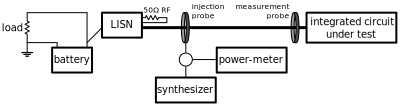
\includegraphics[width=\textwidth]{src/1/figures/bci_setup.pdf}
  \caption{Bulk Current Injection setup}
  \label{fig:bci-setup}
\end{figure}

% Summary
In summary of the case studies, multiple soft-failures of integrated circuits were studied.
They involved core CMOS logic, SDRAM memories, video processors or multimedia devices failing to work temporarily, detected by raising a flag, display issues and communication errors.
Overall, it was demonstrated that it remains highly difficult to identify the root cause of the failure, especially without access to the design of the chip.
A multitude of tools has been employed throughout the studies, such as near-field injection and scan, modified TEM cells, SPICE and electromagnetic simulations and modeling languages such as VHDL-AMS.
Ultimately, it seems that access to the silicon design is essential to debug the problem and fix, as was shown successfully in \cite{softfailEMCIC}.
All these conclusions call for new investigation methods at silicon level, and modeling method for enabling system level simulations without disclosing intellectual property.
The new methods and tools presented in this document aim to solve exactly this kind of issues.

\subsection{Observation methods}

F. Caignet proposes in \cite{eq-time-sampling} an on-chip measurement technique capable of recording \gls{esd} waveforms with a \SI{20}{\giga\hertz} bandwidth.
It relies on equivalent-time sampling for measuring waveforms with a much larger bandwidth that real-time oscilloscopes.
Equivalent time-sampling works exclusively with repeatable or periodic signals.
A real-time oscilloscope takes a complete waveform constituted of \textit{N} samples in a single shot.
On the other hand, a time-equivalent sampler measures waveforms point by point, and require \textit{N} repetitions of the waveform to acquire the \textit{N} samples.
The process for acquiring the data is the following.
A first waveform is shot, and the sampler only records its value at $t=0$.
A second waveform is shot, and the sampler records the value at $t=\Delta t$.
At the third waveform, the recording is at $t=2\Delta t$.
The process is repeated while increasing the sampling delay by \textDelta{}t at each step until enough points were acquired.
This approach is interesting because it reduces a lot the constraints on the measurement system, while offering a huge bandwidth.
The main disadvantage is that it requires as many measurements as the amount of points needed.
In \cite{eq-time-sampling}, the sampler was designed using a CMOS \SI{65}{\nano\metre} technology and embedded into a testchip.
Architecture is given in Fig. \ref{fig:eq-time-sampler-architecture}.

\begin{figure}[!h]
  \centering
  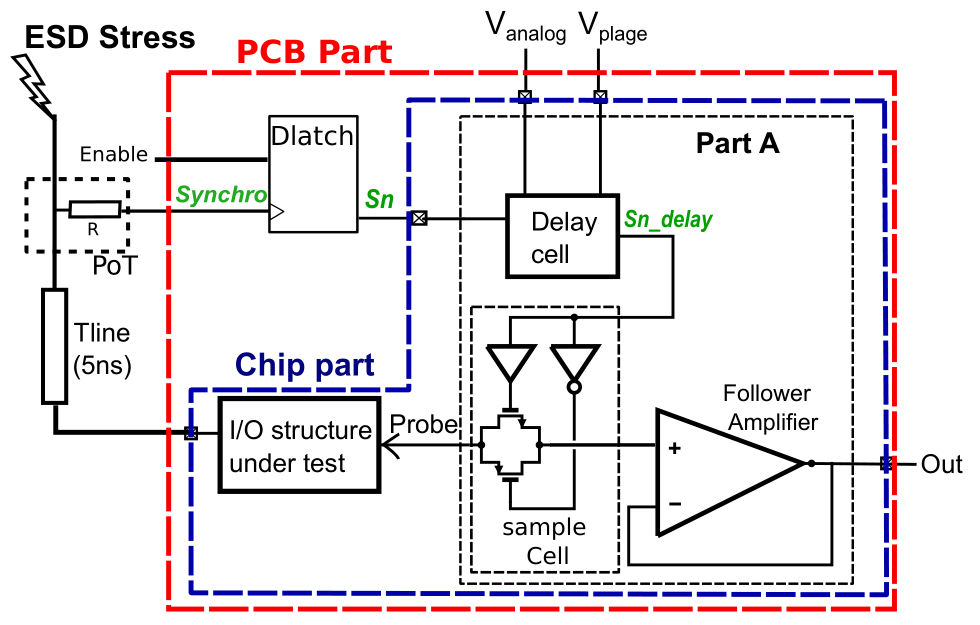
\includegraphics[width=0.6\textwidth]{src/1/figures/architecture_equivalent_time_sampler.png}
  \caption{Equivalent time-sampler architecture from \cite{eq-time-sampling}}
  \label{fig:eq-time-sampler-architecture}
\end{figure}

Other techniques exist in similar fields that could prove useful for ESD investigation.
M. Nagata details in \cite{substrate-noise-measurement} an on-chip measurement technique for recording substrate noise waveforms at silicon level.
Injection and measurement structures are directly integrated into a \SI{0.4}{\micro\metre} CMOS technology test vehicle.
The injection structures consists in a controllable noise source.
The amount of logic elements, transition directions and delays can be selected to generate different noise waveforms.
By coupling, the substrate receives a part of this disturbance.
The sensor consists in a latch comparator \ref{fig:noise-detect-latch-comparator}.
With a few synchronization signals, it is sufficient to record waveforms with a \SI{100}{\pico\second} time resolution.
For \gls{esd}, this sampling frequency is almost ideal.

\begin{figure}[!h]
  \centering
  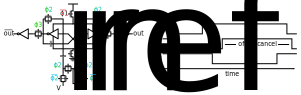
\includegraphics[width=\textwidth]{src/1/figures/latch_comparator.pdf}
  \caption{Latch comparator and timings for substrate noise detection from \cite{}}
  \label{fig:noise-detect-latch-comparator}
\end{figure}

\subsubsection{Emission Microscopy (EMMI)}

% Concept
\gls{emmi} is an observation technique where a camera registers photon emission above semiconductor devices.
A device is placed in the field of view of the camera.
The entire system is placed inside an enclosure to block out all ambient light.
Semiconductor junctions and defects emit photons when electrically excited.
By letting the camera shutter open for a long time, between a few hundred milliseconds to tens of seconds, photons generated by this process are detected by the image sensor.
As photons accumulate, some sections of the image become brighter than others.
Defects can be isolated from normal junctions by comparing recordings performed on tested devices with a reference device.
The architecture of an \gls{emmi} system is provided in Fig. \ref{fig:emmi}.

\begin{figure}[!h]
  \centering
  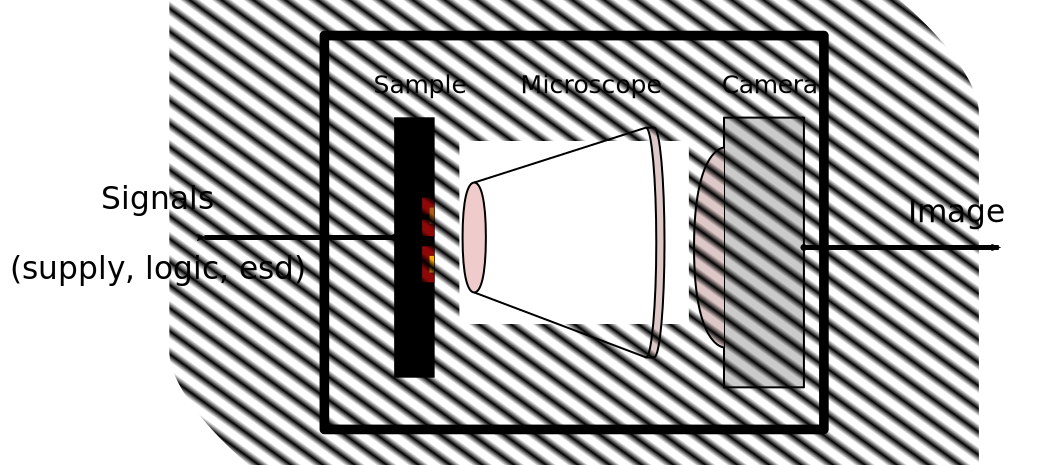
\includegraphics[width=0.8\textwidth]{src/1/figures/architecture_emmi.pdf}
  \caption{Architecture of an emission microscopy testbench}
  \label{fig:emmi}
\end{figure}

% In ESD field, how was used EMMI
Originally, the combination of \gls{emmi} with a \gls{tlp} discharge was proposed by T. Maloney and N. Khurana in the original TLP paper \cite{TLP}.
Afterwards, EMMI was employed for debugging hard-failures of ESD protections in 3D CMOS technologies \cite{kessler2002method} or high-voltage silicon technologies \cite{emmi-tlp}.
In US patent 6469536 \cite{kessler2002method}, Kessler describes a method to synchronize the ESD injection with the shutter of the EMMI.
Finally, \gls{emmi} is presented in \cite{softfailEMMI} as a successful analysis method for debugging and locating a functional failure on an integrated circuit exposed to \gls{esd}.
In this last paper, the integrated circuit is powered-on and in normal operation, and the \gls{emmi} helps localize soft-failures.

% Show examples
Fig. \ref{fig:emmi-examples} shows two different images recorded with an \gls{emmi} bench.
The image on the left is the reference image and the one on the right is the signature after a failure.

\begin{figure}[!h]
  \centering
  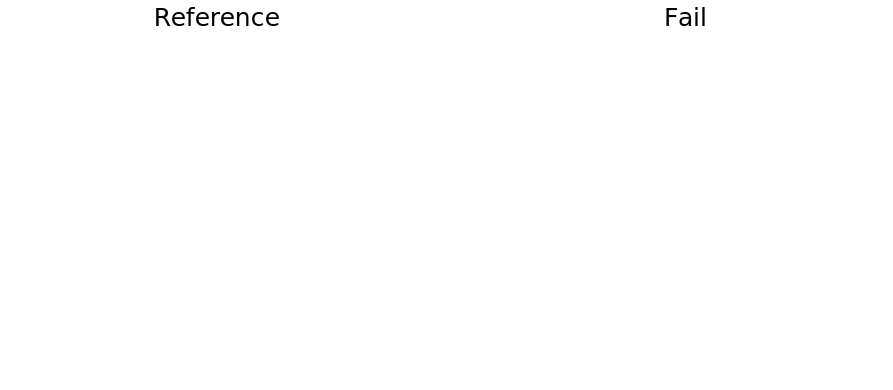
\includegraphics[width=\textwidth]{src/1/figures/emmi_comparison.pdf}
  \caption{reference and fail EMMI measurement of an integrated function}
  \label{fig:emmi-examples}
\end{figure}

\subsubsection{Near-field scanner}
\label{sec:near-field-scan}

% Introduce near-field scanner
Electromagnetic near-field scanner allows creating maps of electric and magnetic field.
An electric or magnetic probe is swept closely above a device to record the emitted field in near-field conditions.
Measurements may be carried out in the frequency domain or in the time domain.
This tool was initially intended for architectural analysis such as floor-planning and power distribution analysis.
For ESD, spatial information provided by the recorded map is very useful to locate failures and malfunctions.
A comprehensive and detailed analysis of near-field antennas is done by A.D. Yaghjian in \cite{nfsFirstStudy}.
More recent work details the principle of operation, data processing and hardware requirements in \cite{near-field-scan, planarNFSAntenna, NFSMeasurements, NFScanner}.
Finally, measurement of electromagnetic emissions with surface scan method is standardized in IEC TS 61967-3 \cite{iec61967}.
The architecture of a near-field scanner is given in Fig. \ref{fig:near-field-scanner}.

\begin{figure}[!h]
  \centering
  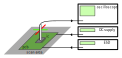
\includegraphics[width=0.7\textwidth]{src/1/figures/architecture_near_field_scanner.pdf}
  \caption{Architecture of a near-field scanning testbench}
  \label{fig:near-field-scanner}
\end{figure}

% Challenges
In a near-field scan, the amplitude recorded by the probe depends on many factors.
The amplitude measured from the sensor is the result of coupling between the source of emission and the sensor itself.
In the case of a magnetic sensor constituted of a loop, the size of the loop, the diameter of the wire, the orientation of the loop and the amount of turns all impact strongly the measured waveform.
Those characteristics can be estimated or measured.
However, the waveform also depends on other factors harder or impossible to determine.
For instance, the height between the emission source (usually a metal track) and the probe and the width of the track affect the coupling ratio.
For realistic integrated circuits, there can be a dense network of metal tracks that all will emit electromagnetic radiations and couple to the sensor.
It is impossible to measure each track independently.
Ultimately, determining absolute values of current or voltage inside a particular portion of an integrated circuit is nearly impossible.
This is why near-field scanners are more interesting for obtaining relative values between different sections of the circuit.
For instance, knowing that the magnetic field above a given structure is ten times greater than another structure is a precious information for understanding ESD propagation.

% Future work
So far, near-field scans are performed mostly at the \gls{pcb} level.
A new trend is to use scanners for integrated circuits.
In current silicon technologies, transistors are a few micrometers long, and metal tracks without power a few micrometers wide as well.
This range of dimensions is to compare with the capabilities of current near-field scanners.
Spatial resolution of a near-field scanner is not bounded by the 3-axis that moves the probe, but by the probe itself.
3-axis machines can easily be found with a positional accuracy of a micrometer, less than the typical observable structure dimensions on silicon.
However, spatial resolution of current near-field probes is more in the range of \SI{100}{\micro\metre}.
This value depends mainly on the size of the loop, its diameter and the distance between sensor and source.
For integrated circuits, this is not sufficient to isolate and identify structures.
In the future, improvements can be expected on the spatial resolution, but it will raise new kinds of challenges.
In the case of a probe with a resolution near \SI{1}{\micro\metre}, the amount of points to record to build the map becomes huge.
For a \SI{5}{\milli\metre} by \SI{5}{\milli\metre} silicon circuit sampled every micrometer, scanning the entire area requires 2.5 million ESD pulse injection and recordings.
No integrated circuit can sustain such an amount of repeated stressing, and the device will be destroyed before the end of the scan.
Also, the test time for this brute force approach is going to be very important.
If the entire process is automated and a delay of 2 seconds is left between each point, the test campaign will still take 1388 hours, approximately 2 months.
With smarter sampling strategies or new measurement methods, near-field scanning could be a valuable tool for silicon-level investigation.

% Near-field scan as injection tool
So far, near-field scan has been presented as a measurement tool, but it can also serve as a localized stress injection system.
Instead of sensing voltage or current in the near-field probe, a pulse is injected in it.
In \cite{NearFieldInjectionFabrice}, a near-field scanner is combined with a very fast \gls{tlp}.
A stress is injected, and the device under test is monitored for faults.
A susceptibility map is obtained \ref{fig:near-field-scan-map}, that highlights the most sensitive areas of a board.
The paper demonstrates that it is possible to map quantitatively and with good resolution the \gls{esd} susceptibility of a board with this method.
In a similar approach, \gls{esd} sensitive metal tracks and \gls{ic} pins are identified in \cite{NearFieldInjectionBis} using a near-field scanner as an injection system.

\begin{figure}[!h]
  \centering
  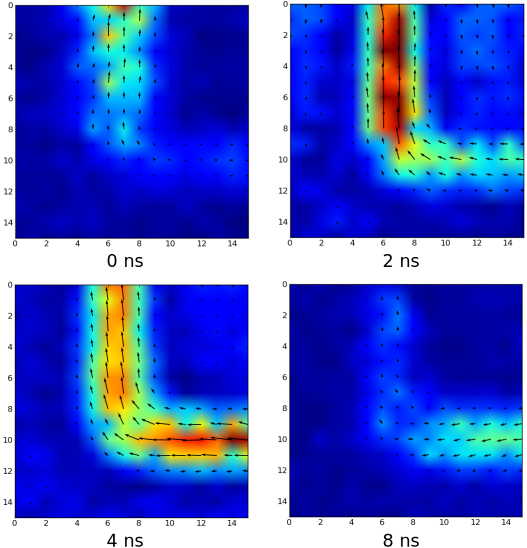
\includegraphics[width=0.9\textwidth]{src/1/figures/nfs_map.pdf}
  \caption{Near-field injection susceptibility map \cite{phd-monnereau}}
  \label{fig:near-field-scan-map}
\end{figure}


\subsection{Modeling methods of soft-failures for integrated circuits}

In the literature, various ESD modeling methods can be found.
They comprise a wide range of techniques such as 3D electromagnetic and semiconductor physics simulations, compact, behavioral, physically-based and non-linear modeling.
The methods described hereafter could be used for soft-failure investigation.

M. Scholz details a mixed-mode ESD simulation approach in \cite{mixedModeESDSims}.
It is a combination of \gls{spice} and \gls{tcad} models, simulated in \gls{spice} environment.
The author indicates that the combination of physical device models and standard simulations provides higher accuracy and more realistic simulations than behavioral \gls{spice} models.
Using this complex simulation tool, on-chip and off-chip device interactions are studied, in powered and unpowered conditions.

In \cite{usb2ESDProtection}, TLP characterizations serves as an I(V) model for both external protections and an \gls{ic} pin.
The \gls{pcb} S-parameters are extracted from the board layout, using Momentum software (Agilent Technology).
It is electrically model with lumped R,L,C,G elements.
The modeling approach proved successful for simulation interactions between external devices and on-chip structures.
This method is interesting for soft-failure analysis because it is thorough and complete and enables accurate ESD simulation.

% IBIS is not enough for modelling an IC pin for ESD simulations
The Input Output Buffer Information Specification (IBIS) \cite{ibis-spec} is a behavioral, black-box model for performing signal integrity simulation on digital circuits.
It is widespread in the digital \gls{asic} world because it enables accurate simulations without disclosing circuit or process information.
It was envisioned that IBIS models could also be used or extended for ESD.
It is demonstrated in \cite{ibisImprovementFabrice} that the model lacks some parameters for EMC and ESD simulations.
It comprises a current versus voltage characteristic of \gls{io}s, similar to what can be extracted by a TLP, however the IBIS model is not defined for fast pulses and high injection.

N. Lacrampe proposes in \cite{LacrampeTransientImmunity} to perform 3D electromagnetic simulations at silicon level, using the integrated circuit layout, to deduce the amount of capacitive couplings between Vdd and Vss rails.
The extraction is performed with HFSS software (Ansoft).
The goal of this analysis is to predict the susceptibility of integrated circuits against electrostatic discharges.
\gls{pcb} tracks are modeled by a distributed RLC network.
The package data from the IBIS model \cite{ibis-spec} was used in the simulations.
Finally, a TLP stress generator is modeled using a lookup table I(V) component, in series with a \SI{50}{\ohm} resistor.

Once again, electromagnetic full-wave simulations are conducted in powered-on ESD analysis in \cite{softFailMobile}.
System-level components are simulated, such as PCB, metallic casing and battery pack.
3D EM simulations helps identify the main discharge paths and locate the failure.


\chapter{Electrical modeling methods of integrated circuits for ESD}

\section{System-level modeling}

Simulations are a great tool to get a better understanding of the impact of \gls{esd}s on integrated circuits.
They allow introspection inside specific nets of the circuit, observe behavior that would be hard to observe in the field.
However, \gls{esd} simulations are not common practice and must be validated against measurement data before being used as an investigation tool.
Models for key devices must be derived, at each scale of the system.

In this chapter, the methodology for building models at the system level is detailed.
It mostly targets ESD generators and lab equipment.

\subsection{Lossless transmission lines}

\gls{esd} events generally last a few hundred nanoseconds.
At this timescale, delays introduced by usual coaxial cables found in labs and metal traces on \gls{pcb} are no longer negligible.
Depending on the configuration, these delays can generate oscillations, amplitude variations.

Most cables and PCB traces, although of very different construction, usually behave as lossless transmission lines.

A transmission line is defined by two key parameters, its \gls{Zc} and propagation delay.
Alone, these two parameters can be used in a behavioral model to describe efficiently and with great accuracy the behavior of lossless transmission lines.

The electrical model is constituted of two voltage-controlled voltage sources and two resistors.
Compared to the classic RLC distributed model, the behavioral model has infinite bandwith, and constant complexity (compared to RLC where the amount of elements increases with the required bandwidth).

ELECTRICAL MODEL

EQUATIONS

\section{IC level ESD modeling}

Sub section


\chapter{Study of soft-failures at silicon-level}

\section{Study of a real product}
\label{sec:study-real-product}

Hello

\section{Test vehicle}
\subsection{Test vehicle description}
\label{sec:test-vehicle-desc}

% A testchip has been made to put measurement structures on silicon
Integrated circuits are very dense and fragile devices, enclosed in plastic or ceramic packages.
It is nearly impossible to measure electrical properties without physical access.
For instance, it could be useful to measure potential inside a given net inside the circuit.
With integrated circuits, this is not doable and most of the time the external connections are the only points of access.
Even with physical internal access, placing micro-probes to contact metal connections can disturb sensitive parts of the device.
To overcome these issues, new approaches are required.
In this research, custom measurement structures have been implemented directly on-chip.
They perform analog measurements at the silicon level.

\begin{figure}[h]
  \centering
  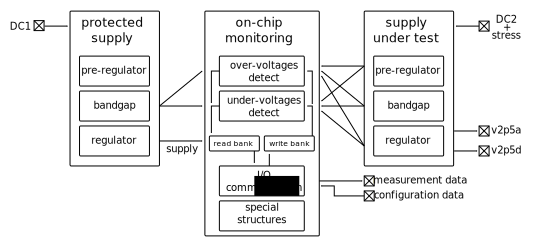
\includegraphics{src/3/figures/architecture_testchip.pdf}
  \caption{Global architecture of the test vehicle}
  \label{architecture_testchip}
\end{figure}

The global architecture of the testchip is provided in Fig. \ref{architecture_testchip}.
It contains two instances of the regulation function studied earlier in \ref{sec:study-real-product}.

% Right supply
The first instance (right side of Fig. \ref{architecture_testchip}) is exposed to \gls{ESD} stresses during tests.
It is monitored in multiple points by the measurement and monitoring structures.

% Left supply
The second instance powers the monitoring functions and communication buses.
It must not be disturbed by the discharges injected during testing on DC\textsubscript{2}.
It has its own external supply pin DC\textsubscript{1}, isolated from DC\textsubscript{2}.
Large external filtering and decoupling capability has been setup on DC\textsubscript{1}.
Except for the ground connection, the two regulators do not share connections.

% What is in the monitoring system
The on-chip monitoring system is composed of several overvoltage and undervoltage detectors.
They monitor voltages of multiple nets inside the supply under test.
There are in total 9 detectors in the testchip.
5 of them are dedicated to preliminary testing and self-validation, and are not actually monitoring analog blocks.
The 4 remaining blocks are monitoring the regulator under test (Table \ref{tab:detectors}).
Threshold can be configured externally using a communication bus.
When new value is set through the communication, a digital to analog converter generates the new threshold for each detector.
The detectors are able to detect level crossings from half a volt up to 13 V, which is designed to match the voltage range of most signals inside the chip.

\begin{table}[!htbp]
\centering
\begin{tabular}{@{}lll@{}}
\toprule
Name           & Nominal value & Function \\ \toprule
uv\_9V	       & 9V   & undervoltage detect on v\textsubscript{clamp9} (settable threshold)\\
ov\_9V	       & 9V   & overvoltage detect on v\textsubscript{clamp9} (settable threshold)\\
ov\_vref1p2	   & 1.2V & overvoltage detect on bandgap reference (settable threshold) \\
uv\_vref1p2	   & 1.2V & undervoltage detect on bandgap reference (settable threshold) \\
\bottomrule
\end{tabular}
\caption{Detectors on core functions}
\label{tab:detectors}
\end{table}

% What is in the communication system
The communication buses provide a connection between the internal detectors and the external world, using digital \gls{io}.
Configuration data can be provided from an external microcontroller and measurement data is output by the communication block.
There are two readable buses and two writeable buses.
The first read and write buses are used for preliminary validation of the on-chip monitoring.
The complete register maps in read and write mode are given in appendix \ref{apx:testchip-register-maps}.

% How those monitoring functions have been designed
The implementation of each monitoring function is detailed hereafter.

\subsection{Voltage monitoring}

% What are the OV/UV detectors made of
Overvoltage and undervoltage detectors are built with latched comparators.
A flag is raised if a monitored net crosses a threshold, and stored using a latch, until it can be read.
The architecture of a single detector is given Fig. \ref{fig:architecture-ov}.
The same architecture is used for the overvoltage and the undervoltage.
Monitored and reference inputs are just inversed on the undervoltage detector.

\begin{figure}[!h]
  \centering
  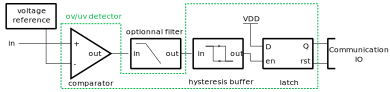
\includegraphics[width=0.9\textwidth]{src/3/figures/architecture_OV.pdf}
  \caption{Architecture of the overvoltage detector}
  \label{fig:architecture-ov}
\end{figure}

% Detail architecture
The first block in this detector is the comparator.
It is designed with a two-stage operational amplifier with an output buffer (see Fig. \ref{fig:comparator-design}).
This topology is well suited for high-gain, open-loop comparators.
This comparator provides a very high input impedance, to ensure the monitored net is not disturbed.
A high-gain is useful for limiting the comparator's offset and to ensure that the comparison will be accurate.
The offset of the designed comparator is below 5 mV and the switching speed under 20 ns (on a 50pF load), which should be sufficient to detect fast glitches of several volts amplitude and a timescale similar to electrostatic discharges.

\begin{figure}[!h]
  \centering
  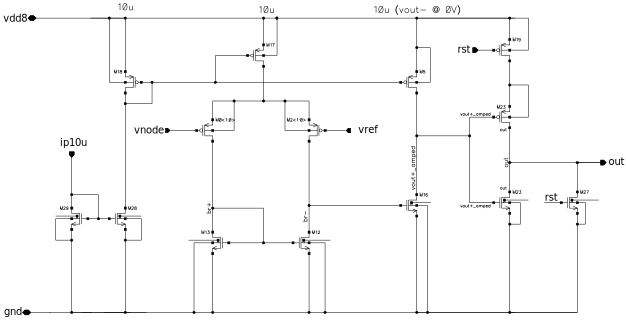
\includegraphics[width=0.9\textwidth]{src/3/figures/comparator_design_clean.pdf}
  \caption{Comparator design}
  \label{fig:comparator-design}
\end{figure}

% What is the purpose of filter
On the output of the comparator (Fig. \ref{fig:architecture-ov}), an optional RC filter can be connected.
This filter can deglitch very short overvoltages, to only let large overvoltages pass through the detector.
The stratety behind this filter is to use multiple detectors monitoring the same net, each one with a different filter.
In function of which detectors triggered, an estimation of the overvoltage length can be made.

% Hysteresis buffer
After the filter, an hysteresis buffer guarantees that a clean digital signal will be fed to the latch.
The triggering levels are set quite far away, with the low level near 2V and the high level at about 6V.

% Latch
Finally, the latch stores the overvoltage flag.
By default it stores a low-level.
Its copy input $D$ is connected to the supply.
If the hysteresis buffer triggers high, the enable pin triggers a copy in the latch.
The output $Q$ copies the value from the $D$, storing a logical high in the latch.
This way, any detected overvoltage or undervoltage is stored until it can be red or the latch is reset.

% Origin of reference voltages
The reference voltages for these comparators come from either fixed-values set by the protected supply, or \gls{dac} that can be reconfigured through the communication system.

\subsection{Communication system}
\label{sec:comm-system-testchip}

% Why a comm IO
The manufacturing process at NXP for test vehicles requires a 48 pin package.
On those 48 pins, a few are already required for ground connection and substrate connection.
Also, the two instances of the regulation function each need a supply connection and two external decoupling capacitors.
The on-chip current sensor also require 4 pins for the calibration pattern and two pins per actual sensor.
In the end, the available pin count would be too small for allowing to connect each detector to its own external pin.
To overcome this issue, a custom communication bus has been designed, to discuss with the testchip before and after ESD tests.
Initially, the JTAG (Joint Test Action Group) \cite{jtag} protocol was envisionned for this application.
It is a test port for access and boundary-scan.
It is commonly used to check that connections are correct between integrated circuits, and to configure internal parameters such as trim values and internal fuses.
However, the JTAG system needs a digital state-machine for operation, described in any hardware description language (HDL).
This step requires digital-synthesis, a step that converts a HDL sources into electrical netlist.
Given the resource constraints in this research work, this step was not available for this test vehicle.
Instead, a simplified serial to parallel protocol has been designed from scratch.
The main idea to design reusable communication cells that can be duplicated and connected in a chain fashion, to get a register map of any size easily.
Changing the size of the register is simply a matter of adding or removing individual cells.
No digital-synthesis is being required.

% Overall architecture
The chain of individual cells functions by propagating from cell to cell an enable signal.
Each time a cell receives the enable signal, it will perform its task, then pass the enable to the next cell at the next clock edge.

\subsubsection{Read cell}

% Explain behavior
The read cell is constituted of a tri-state buffer and a D-latch (see Fig. \ref{fig:read-cell-design}).
The output of the tri-state buffer is set in high-impedance when input \textit{x} is low.
This action releases the communication bus for other read cells and is the default state.

\begin{figure}[!h]
  \centering
  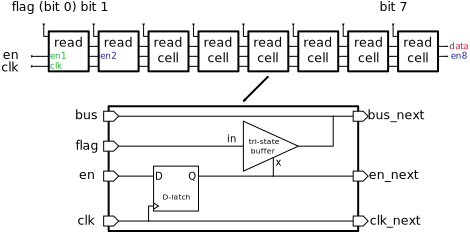
\includegraphics[width=0.8\textwidth]{src/3/figures/architecture_read_cell.pdf}
  \caption{Read-only cell design}
  \label{fig:read-cell-design}
\end{figure}

% Describe the chronogram
Fig. \ref{fig:read-cell-curve} shows the simulated behavior of a chain of 8 reading cells.
Signals in green (\textit{en1} and \textit{clk}) must be provided externally, by a microcontroller for instance.
Signals in blue (\textit{en2} and \textit{en8}) are internal control signals, to help the cells determine if they have the right to write on the bus.
The signal in red (\textit{data}) is the data output, read by an external microcontroller.

% Explain time-response
The reading sequence is initiated by setting \textit{en1} high.
When \textit{en1} is set high, the output of the first latch (\textit{en2}) switches high at the next clock cycle.
This means the first cell has the permission to write on the bus.
During one clock cycle, the \textit{flag} is written on \textit{data} bus.
At the next clock cycle, the enable signal is propagated to the next cell.
The first cell no longer has the permission to write to the bus.
The second cell writes to the bus, during a single clock cycle.
The process is naturally repeated by the system, until the enable has been propagated to the last cell (\textit{en8}) and all serial data was written.

\begin{figure}[!h]
  \centering
  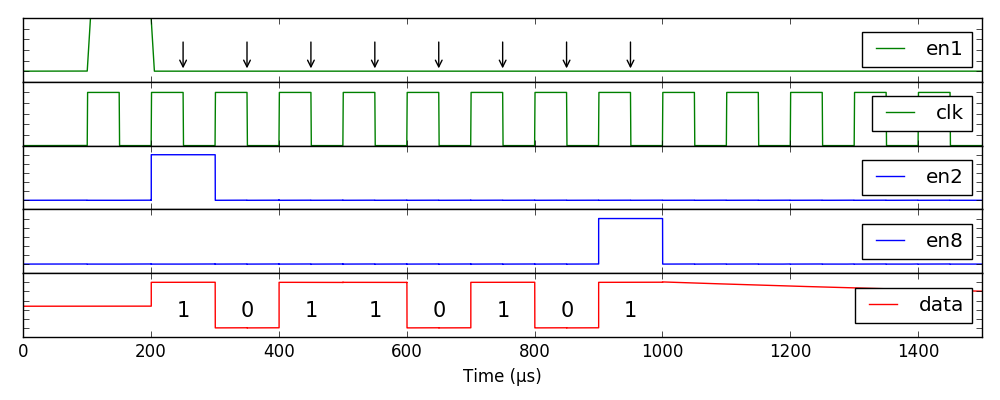
\includegraphics[width=0.95\textwidth]{src/3/figures/curve_read_cell.png}
  \caption{Chronogram for the read cell}
  \label{fig:read-cell-curve}
\end{figure}

\subsubsection{Write cell}

% Explain behavior
The write cell is a bit more complex but operates on the same principle (Fig. \ref{fig:write-cell-design}).
Data is placed serially by the user on the \textit{bus} line, syncronously with the clock.
The enable signal is propagated from cell to cell, so that each cell knows when to sample the bus line and store the value.
Basically, this cell sets on its \textit{output} the value on the bus when its enable is high (Fig. \ref{fig:write-cell-curve}).

\begin{figure}[!h]
  \centering
  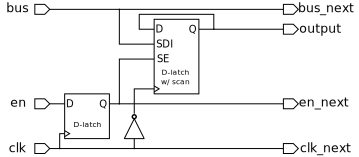
\includegraphics[width=0.8\textwidth]{src/3/figures/architecture_write_cell.pdf}
  \caption{Write-only cell design}
  \label{fig:write-cell-design}
\end{figure}

% Detail devices
The truth table of this latch is given in table \ref{tab:d-latch-scan-truth}.
D1 is a synchronous D-latch.
The output Q copies the input D on rising clock edges.
D2 is a synchronous D-latch with scan.
The output Q copies the data input D on rising clock edges, storing a value.
When the scan enable \textit{se} input is HIGH, the data input D copies the value of the scan data input (\textit{SDI}), effectively changing the stored value.

\begin{table}[!h]
\centering
\begin{tabular}{@{}lllll@{}}
\toprule
D  &  SDI  &  SE  &  CLK  &  Q \\ \midrule
0  &  -    &  0   &  \nearrow    &  0 \\
1  &  -    &  0   &  \nearrow    &  1 \\
-  &  0    &  1   &  \nearrow    &  0 \\
-  &  1    &  1   &  \nearrow    &  1 \\
-  &  -    &  -   &  \searrow    &  Q \\
\bottomrule
\end{tabular}
\caption{D-latch with scan truth-table}
\label{tab:d-latch-scan-truth}
\end{table}

\begin{figure}[!h]
  \centering
  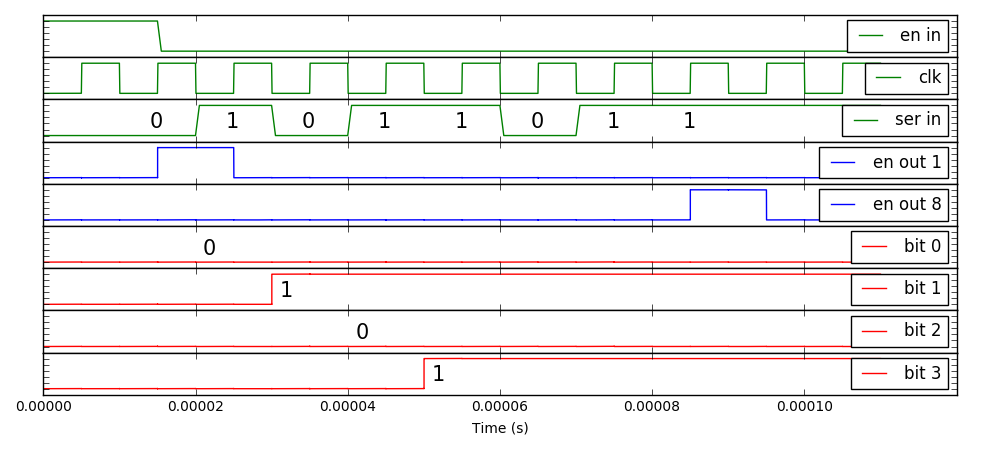
\includegraphics[width=0.95\textwidth]{src/3/figures/curve_write_cell.png}
  \caption{Chronogram for the write cell}
  \label{fig:write-cell-curve}
\end{figure}

% Describe the chronogram
Fig. \ref{fig:write-cell-curve} shows the simulated behavior of a chain of 8 writing cells.
Signals in green (\textit{en1} and \textit{clk}) must be provided externally.
Signals in blue are internal control signals, to help the cells determine if to who belongs the data on the bus.
The signals in red (\textit{bit 0} to \textit{bit n}) are the data output, set on each individual output bit.
Ultimately, the reading-cell performs a serial to parallel conversion.
The serial data is set on \textit{bus}, and the parallel outputs are \textit{bit 0} to \textit{bit n}.

\subsection{On-chip near-field current sensors}

% Measuring currents is important too
Current sensing magnetic loops were integrated on silicon to measure current trough a few critical nets.
They are sensitive to currents circulating nearby, and were placed close to metal tracks in which current must be measured.
By coupling, the sensor generates a voltage proportional to the derivative of the current in the track.
Figs. \ref{fig:near-field-current-sensor} and \ref{fig:near-field-current-sensor-layout} give respectively a visual representation of the metallic loop and its layout.
This kind of integrated loop was studied in \cite{OtherInductors, InductorsLAAS1, InductorsLAAS2, AlainSallesInductors}.

\begin{figure}[!h]
  \centering
  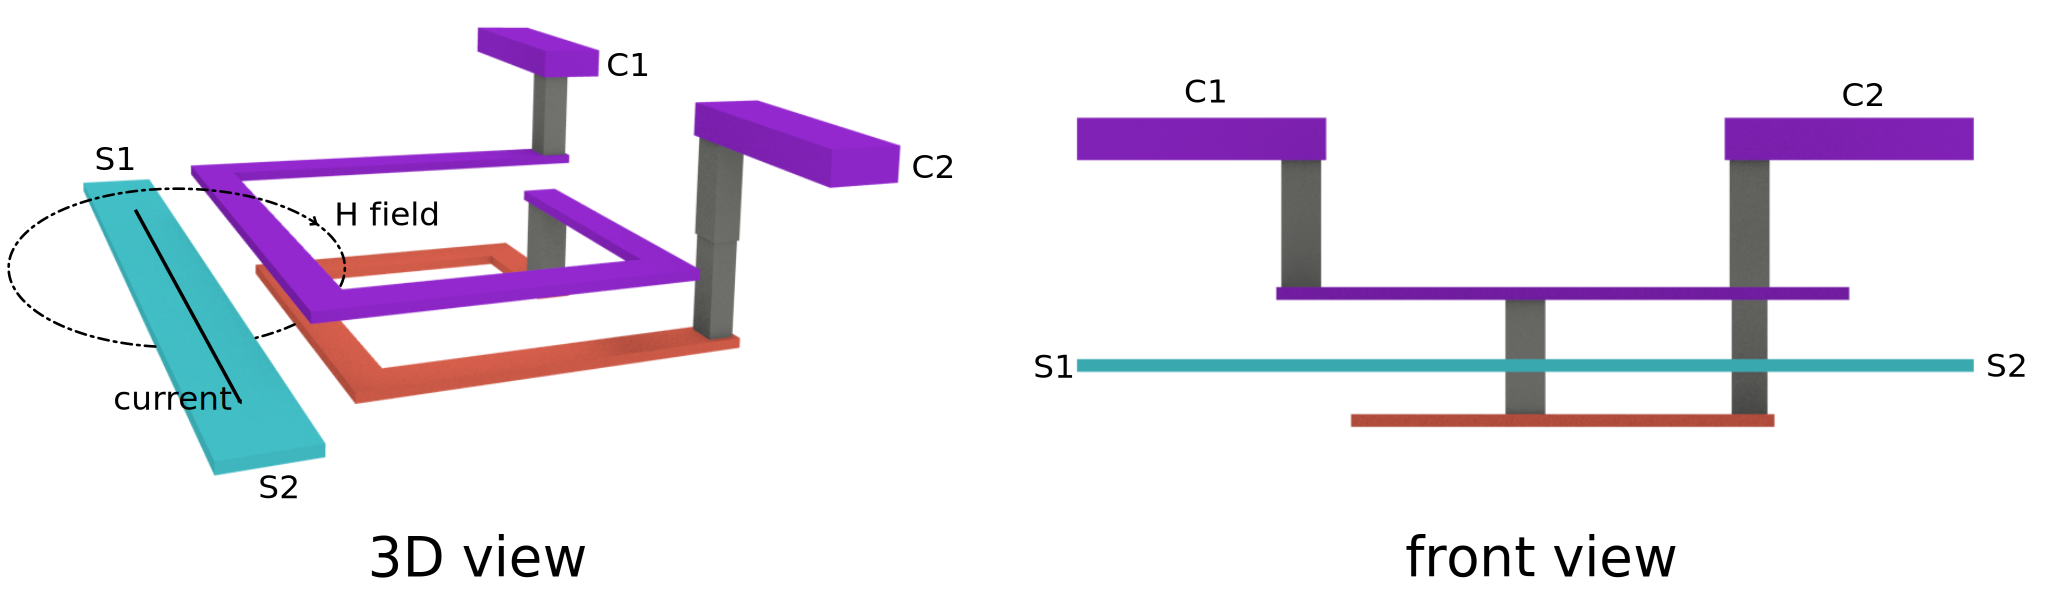
\includegraphics[width=0.98\textwidth]{src/3/figures/near-field-current-sensor.pdf}
  \caption{Near-field current sensor design}
  \label{fig:near-field-current-sensor}
\end{figure}

\begin{figure}[!h]
  \centering
  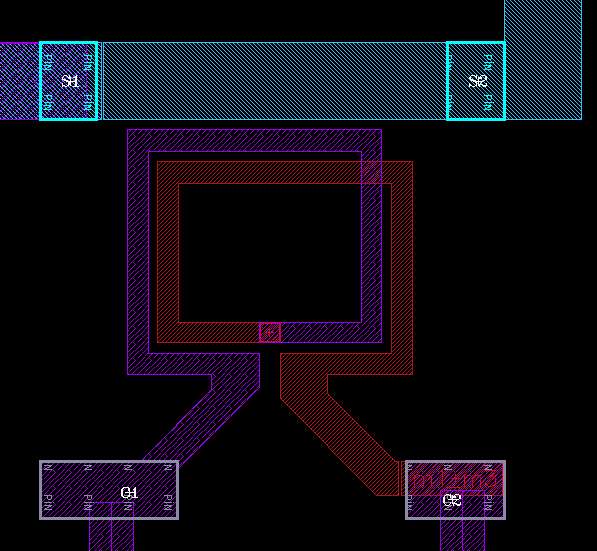
\includegraphics[width=0.5\textwidth]{src/3/figures/sensor_layout.png}
  \caption{Near-field current sensor layout}
  \label{fig:near-field-current-sensor-layout}
\end{figure}

% How is it designed and how is it used
On silicon, three levels of metal are used to build the loop.
The first level (in red) and the third level (in purple) form a circle.
Metallic vias connect both levels to close the loop vertically.
Finally, the sensed current is at the second level (pale blue), and circulates between nets \textit{S1} and \textit{S2}.
An oscilloscope with 50\textOmega{} input impedance performs a differential voltage measurement between pins \textit{C1} and \textit{C2}.
An example waveform obtained by injecting a rectangular pulse is given in Fig. \ref{fig:nfs-wvf}.
The obtained waveform requires specific post-processing to reconstitute the original current waveform.
The post-processing is detailed earlier in section \ref{sec:on-chip-near-field-process}.

\begin{figure}[!h]
  \centering
  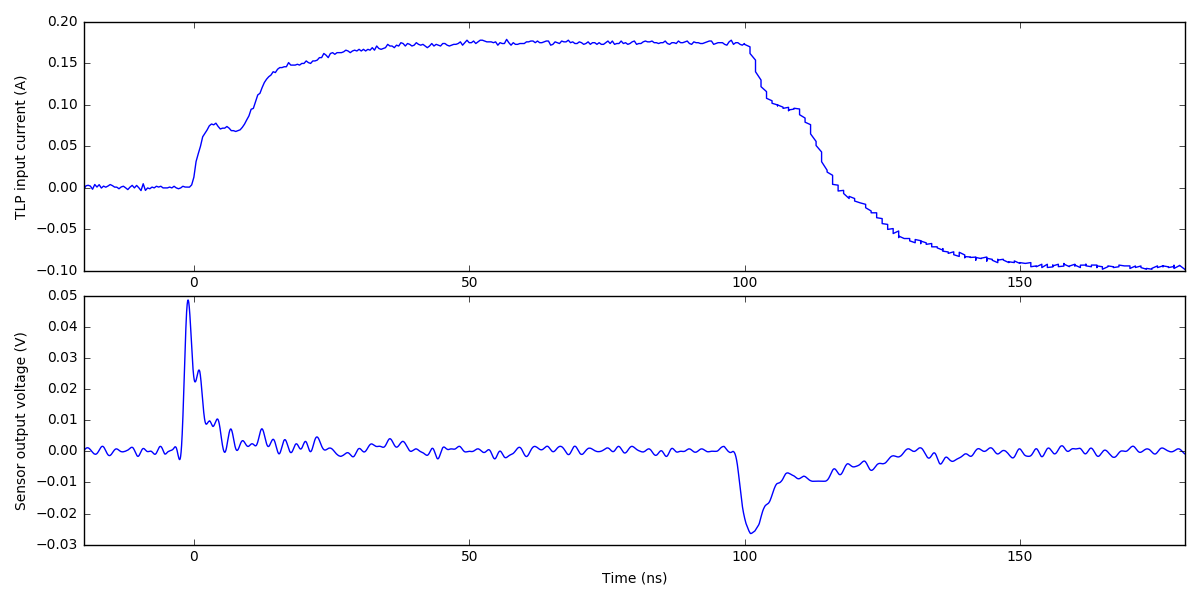
\includegraphics[width=0.9\textwidth]{src/3/figures/measured_waveform.png}
  \caption{Waveform measured with an oscilloscope connected to the on-chip near-field sensor}
  \label{fig:nfs-wvf}
\end{figure}

% Talk about the near-field current sensors placement
In total, there are 6 near-field current sensors located on the device.
The 6\textsuperscript{th} sensor is dedicated to calibration.
The others are placed strategically on main \gls{io} susceptible to be disturbed directly or indirectly by \gls{esd}s.
Sensor \textit{1} measures the current on the supply under test power input.
During testing, this pin is be exposed to \gls{esd}s coupled on top of a DC supply voltage.
Internally, this input is protected by a large \gls{esd-protection}, able to sustain IEC 61000-4-2 \gls{esd-gun} discharges.
Sensor \textit{2} measures the current absorbed and deviated by the \gls{esd-protection} into the \textit{gndsub} metal ring (local ground reference).
Sensors \textit{3} measures the current flowing to the external stabilisation capacitor of the regulator under test.
Finally, sensors \textit{4} and \textit{5} measure the currents flowing from the \textit{gndsub} metal ring into the external ground pins, connected externally to the board ground.

\subsection{Topcell}

%
The primary supply chain under test is directly extracted from a real product, described in \ref{sec:product-desc}.
It is placed in appropriate operating conditions on the testchip, and behaves identically to the real product.
Except for the two supply blocks, all the functionalities described previously were designed, simulated and layouted.
All layouts were assembled together to form the topcell (Fig. \ref{fig:top-cell-layout}).
The complete pinout is given in appendix \ref{apx:testchip-pinout}.

\begin{figure}[!h]
  \centering
  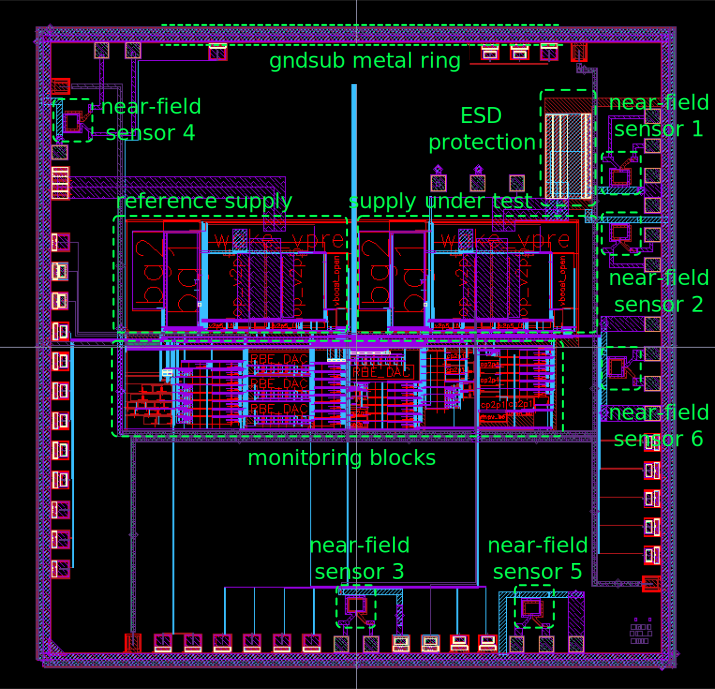
\includegraphics[width=0.7\textwidth]{src/3/figures/topcell_layout.pdf}
  \caption{Top-cell layout}
  \label{fig:top-cell-layout}
\end{figure}

% Explain why so much empty space
On the layout, a lot of silicon space was left empty.
This is due to manufacturing constraints that enforced the silicon dimensions.
After manufacturing and packaging, the chip is tested.
The entire testing process and results are documented in section \ref{sec:test-vehicle-testing}.

\subsection{Test vehicle verification and testing after manufacturing}
\label{sec:test-vehicle-testing}

The testplan for the testchip is constituted of 7 steps, described in Fig. \ref{fig:verif-plan}.
The verification of the on-board voltage regulation is checked with a voltmeter, to ensure that a regulated \SI{12}{\volt} is well established.
The on-chip regulation is checked with a voltmeter and observed with an oscilloscope to validate the behavior.
All regulators from both boards and inside the testchip were found to operate as expected.

\begin{figure}[!h]
  \centering
  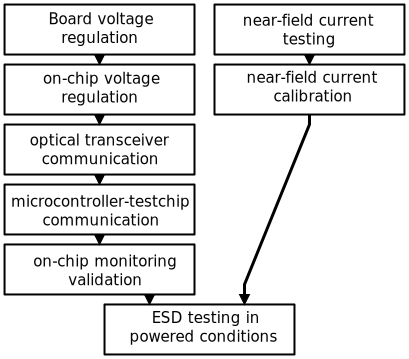
\includegraphics[width=0.7\textwidth]{src/3/figures/verification_plan.pdf}
  \caption{Test plan}
  \label{fig:verif-plan}
\end{figure}


\subsubsection{Optical communication}

% What is this step
The communication between the optical transceiver is verified.
Both the microcontroller and testchip were disconnected prior to injecting test frames on each transceiver.
Then, the output of the matching receiver was observed to ensure that the frame was properly transmitted.
Overall, minor issues were identified and corrected, and the boards were found functional.
This validates the physical layer of the communication.

\subsubsection{Master-slave communication}

The complete communication is then tested.
The microcontroller is used to send command frames such as reading requests on configuration data.
The testchip is supposed to respond each time with some specific data in return.
Unfortunately, very severe issues were found with this system.
After extensive debugging and testing, it was concluded that the communication could not work as-is and needed corrections.
As will be detailed later, the issue did not originally appear in the set of simulations ran during design to validate the entire test vehicle.
It required complex debugging steps such as parasitic devices extraction from layout to only partially reproduce the issue.

% How is the test done
The test is conducted by sending a reading frame multiple times.
By design, the integrated communication system expects a \textit{clk} signal with a frequency lower than \SI{2}{\mega\hertz}, and an \textit{en1} signal that must be high for a single rising clock edge.
With both these criteria met, the communication system should return the data on the \textit{data} pin.

% What is expected
By design, each frame incorporates a few mechanisms to ensure the returned data is correct.
Any \textit{data} frame must start with binary code 1010 and end with binary code 01.
The \textit{en1} signal set on the external input is propagated from one read cell to the next one.
The last cell of the chain is connected to the output pin \textit{en\_out}.
Confidence in the data is increased if the \textit{enable} signal (a pulse with a width of a single clock period) is observed on \textit{en\_out},

% What are the results
After attempting multiple readings with the same board, with different boards and different clock frequencies, the results are inconsistent.
Sometimes, the communication system returns an incomplete frame like in Fig. \ref{fig:read-only-partial-frame}.
In this case, the enable signal is not propagated correctly through the chain.
The \textit{en\_out} signal (not displayed here) stays low all the time.

\begin{figure}[!h]
  \centering
  \includegraphics[width=0.8\textwidth]{src/3/figures/read_only_partial_frame.pdf}
  \caption{Read-only partially returned frame (\SI[per-mode=symbol]{4}{\milli\second\per\div}, \SI[per-mode=symbol]{5}{\volt\per\div}) - clock frequency \SI{1}{\kilo\hertz}}
  \label{fig:read-only-partial-frame}
\end{figure}

In other cases, the chain returns a complete but corrupted frame like in Fig. \ref{fig:read-only-full-frame}.
The enable is correctly propagated, and is visible on \textit{en\_out}, however the data start pattern is not correct (b'1011 instead of b'1010) and some intermediate digital values are not clearly defined.

\begin{figure}[!h]
  \centering
  \includegraphics[width=0.8\textwidth]{src/3/figures/read_only_corrupted_frame.pdf}
  \caption{Read-only corrupted frame (\SI[per-mode=symbol]{4}{\milli\second\per\div}, \SI[per-mode=symbol]{5}{\volt\per\div}) - clock frequency \SI{1}{\kilo\hertz}}
  \label{fig:read-only-full-frame}
\end{figure}

% Potential cause - clock freq
The clock frequency was initially suspected as a root cause for the problem.
Previous measurements were taken for a slow \SI{1}{\kilo\hertz} clock frequency, which is far slower than the upper limit \SI{2}{\mega\hertz}.
Increasing the clock frequency at \SI{10}{\kilo\hertz}, \SI{100}{\kilo\hertz} and \SI{1}{\mega\hertz} did not improve the situation.

% Potential cause - delays
The impact of parasitic delays causing the communication system to malfunction was also suspected.
Multiple simulations of the entire read chain were run by placing large delays in multiple locations.
No failure could be highlighted using this method.

% Potential cause - parasitic RC
Afterwards, RC parasitic device extraction was performed using the layout.
All previous validation simulations were ran, without any success in finding the issue.
For all simulations, the read chain performed correctly.

% Potential cause - susbstrate coupling
Substrate couplings were also suspected.
Some reading issues could be reproduced, but this type of coupling is highly unlikely to happen for clock frequencies of \SI{1}{\kilo\hertz}.

\subsubsection{Future work}

% Multiple bonding diagrams
A second revision of the testchip is planned.
Since the investigation on the communication system is inconclusive, it was decided to remove it until the root cause of failure could be determined.
Instead, detectors will be directly connected to pads, and most test or validation structure will be removed.
To overcome the problem of low available pin count, it is possible to put on silicon more pads than the amount of external pins.
Then, two different bonding diagrams will be made to connect each part of the available pads, to be able to use all detectors.



\chapter{Modeling of IC for operating ESD simulations}

\section{Test vehicule description and failure signature}

This chapter focuses on the functionnal failure caused by an \gls{esd} of an integrated function.
The studied function is the primary supply of a complex automotive \gls{asic}.
This supply plays a critical role in the functionning of the entire product.
It is connected to the battery of the vehicle, and is the first block of the product to start.
It wakes up and powers all other functions inside the integrated circuit.

\begin{figure}[h]
  \centering
  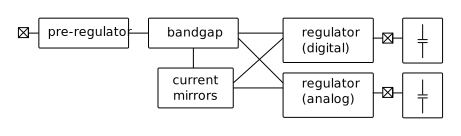
\includegraphics{src/4/figures/testchip_overview.pdf}
  \caption{Architecture of the studied functionnality}
  \label{testchip_overview}
\end{figure}

The primary supply processes the battery supply in a chained fashion (see Fig. \ref{testchip_overview}).
A first block (pre-regulator) clamps the battery voltage (that can reach up to 40V) to 9V, a more acceptable voltage for the silicium technology.
This clamped voltaged is then used to power up a bandgap reference.
Once properly started, this bandgap generates a 1.23 V voltage reference, stable accross a wide range of temperature, process variation and mismatchs.
The bandgap also outputs a 10uA current reference, stable in the same conditions.

After the bandgap, a \gls{ldo} regulator relies on the voltage reference to generate a stable 2.5V supply voltage, able to deliver and sustain up to 20mA.
This first regulator is connected externally to a 100nF decoupling capacitor to absorb peak currents and achieve stability.
This supply is used to supply most analog (digital ?) functions inside the integrated circuit.

A second regulator performs the same task, but starts with a delay compared to the first one.
It also ouputs a 2.5V supply, that powers digital logic inside the circuit.

In case of failure, the primary supply can cause the entire product to shut down.
Indeed, this entire system requires soft-start behavior to avoid generating harmful voltage spikes to powered functions.
This functionnality enforces the system to start on a \br{long} period of time, in the order of a hundred microseconds.

When the system is stressed with an \gls{esd}, voltages and currents are fluctuating inside the block.
Under certain conditions, and especially important stress levels, the block will detects some nodes going in undervoltage or overvoltage.
This will cause the block to go into safe or protected mode, where it will restart because the functionnality cannot be assured properly.
The direct consequence is that the block will require again a hundred microseconds to be again in normal operation mode.

This failure can in a first time be observed in simulation.
An \gls{ESD} is superimposed on the DC battery voltage.
This is the most likely entry point for a stress, because the \gls{IC} exposes a pin to the external workd and is usally connected to the battery via a long cable
To detect is a block reset happened, the voltage on the first voltage regulator is observed.
Fig. X shows the stress waveform on the input.

STRESS WAVEFORM INPUT

Fig. X shows a simulation where a small glitch can be observed on the regulated output, but without clear reset or soft-failure signature.
In this case, the block and the rest of the product is most likely not affected by the ESD.

WAVEFORM OUTPUT NO RESET

Fig. X shows a simulation where a clear reset hapened.
The output voltage is maintained by a 100nF capacitor.
However, it clearly goes down \br{after} the \gls{esd} and rises slowly afterward, a sign that the block went into full reset and restard.

WAVEFORM OUTPUT RESET

By going inside the \gls{IC}...

bandgap, voltage ref, current ref, etc

DISCUSSION AROUND INCREASE OF FAILURE LENGTH after each stage of the chain

\section{Bottom-up block failure modeling}

Consider a system constituted of two blocks A and B connected together.

\begin{figure}[!htbp]
  \centering
  
\includegraphics{src/4/figures/system_ab.pdf}
  \caption{Basic IC function}
  \label{basic_ic_function}
\end{figure}

During normal operation, the \textbf{\textit{out}} signal complies with its specification,
under the condition that the \textbf{\textit{in}} signal does too.
This guarantees that block A and B are performing as expected.

When the system is exposed to an electrical stress on the input during normal operation,
the \textbf{\textit{in}} signal is disturbed.

It no longer complies with its specification, for a given amount of time.

The robustness of the entire system is defined by its ability to maintain signal \textbf{\textit{out}} in specification
while signal \textbf{\textit{in}} is temporarily disturbed.

Time is a key parameter here. On one extreme side, a disturbance that lasts forever is equivalent to the \textbf{\textit{in}} signal not fullfilling its DC specification,
and thus the \textbf{\textit{out}} signal will not fullfill its spec as well.
On the other extreme side, an extremely short disturbance, much shorter than the functionnal timescales of the integrated function will most likely not disturb ??

The first task for defining the robustness of an integrated function is to determine the time threshold under which it can maintain functionnality while being disturbed.
The second key parameter is related to the amplitude of the disturbance, whether it is a voltage, current, energy, etc.
A larger amplitude can make a short pulse more harmful than a lomg one.

\subsection{Block failure characterization and modeling method}

In a bottom-up approach, the study starts on the small-scale components,
later assembled together to reach higher levels of complexity.

This method fits well with the integrated circuit design flow in general,
where blocks are build from transistors and other devices, then assembled together to build interesting functionnalities.

The main perk of this characterization method is its modularity.
Each block can be studied independently.
It complies well with a block-reuse design flow as well.
A characterized block can be reused multiple times without having to re-do the characterization.

Blocks are characterized in a particular setup, and their own robustness is deduced. The final goal is to determine if the robustness of
a system can be assimilated as the sum of the robustness of its parts.

The studied block is placed under normal operating conditions. EXPLAIN MORE.

An input and output pin of interest are selected according to the block's connection inside the chain constituting the total function.
Fix. \ref{block_function_cz} gives an example of such a characterization setup.

\begin{figure}[!htbp]
  \centering
  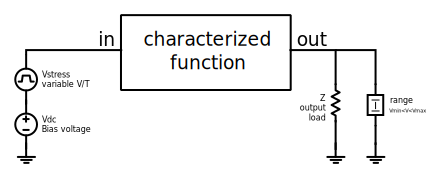
\includegraphics{src/4/figures/characterization_setup.pdf}
  \caption{Block function characterization setup}
  \label{block_function_cz}
\end{figure}

The block is then stressed with a square impulse of variable length and variable amplitude.
Such stress method is called Wunsch & Bell in the litterature (REFERENCE).

The goal is to find out, for each stress duration, what is the minimal voltage \textbf{\textit{V(in)}} required to make the block fail.

Fix. \ref{wb_cz_curve_example} gives an example of such a characterization curve.

\begin{figure}[!htbp]
  \centering
  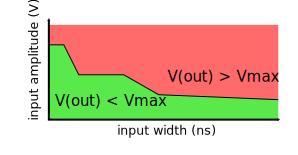
\includegraphics{src/4/figures/example_curve.pdf}
  \caption{Principle of Wunsch & Bell curve for powered-on block testing}
  \label{wb_cz_curve_example}
\end{figure}

The main limitation of this curve is the lack of information on how long the output was disturbed.

If the output is only disturbed for a picosecond, then the failure is most certainly less severe than if it was for a millisecond.

To account for this information, a gradient can be used rather than a simple above/below Vmax curve.
For each point of the curve, the gradient will have a value reprensting the duration of the failure on \textbf{\textit{V(out)}}.
The figure \ref{wb_cz_curve_example_v2} warmer the gradient, the longer the output was disturbed.

\begin{figure}[!htbp]
  \centering
  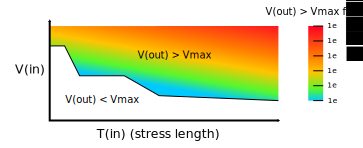
\includegraphics{src/4/figures/example_curve_v2.pdf}
  \caption{Improved curve for Wunsch & Bell powered-on characterization}
  \label{wb_cz_curve_example_v2}
\end{figure}

The gradient can also be discretized into a few aeras for better readability as shown in figure \ref{wb_cz_curve_example_v2_discrete}.
This representation looses some information compared to the gradient one, but is easier to generate and read.
This is the representation we have adopted in the next section, to express the functionnal robustness of a block.

\begin{figure}[!htbp]
  \centering
  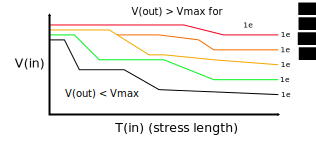
\includegraphics{src/4/figures/example_curve_v2_discrete.pdf}
  \caption{Improved discrete curve for Wunsch & Bell powered-on characterization}
  \label{wb_cz_curve_example_v2_discrete}
\end{figure}

\subsection{Models assembly for full-function robustness}

The method described in section 4.2.1 is performed in simulation-only on the regulation function of the testchip.

This function is composed mainly of three blocks, a pre-regulator, a bandgap and a regulator.

In a first time, a very naive approach is used for the characterization load Z (see figure \ref{block_function_cz}) placed on the output of each block.
An arbitrary load value of 1MΩ is chosen. WHY ?

Like explained previously with Vmax (TO CALL Verr ?) in 4.2.1, a failure treshold is chosen for each block.
Under this threshold, the output of each concerned block is considered at fault.

DETAIL MORE SIMULATION PROCESS. PARAMETERIZED SIMULATION WITH MULTIPLE AMPLITUDE/LENGTH

The characterization curves are given in figs. \ref{pre_regu_wb}, \ref{bandgap_wb} and Z.
For the given testchip, it was found that the regulation function shows clear failure when exposed to negative stresses.
For simplicity, the voltage scale was simply reversed, but this doesn't affect the results in any case.

TODO: REVERT Y SCALE ON ALL CURVES

\begin{figure}[!htbp]
  \centering
  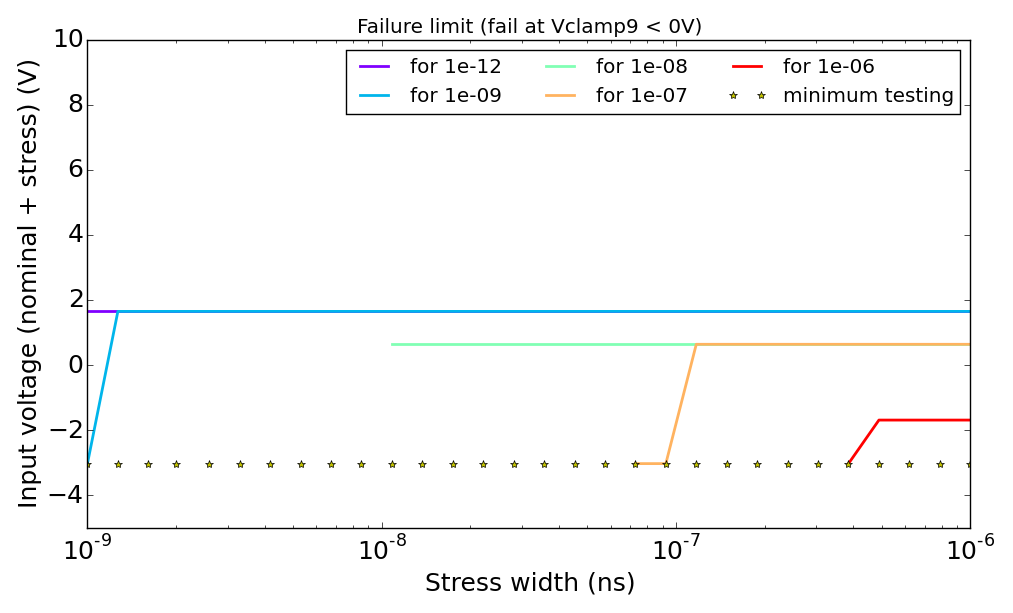
\includegraphics[width=\textwidth]{src/4/figures/cz_vpre.png}
  \caption{Testchip's pre-regulator Wunsch & Bell characterization}
  \label{pre_regu_wb}
\end{figure}

\begin{figure}[!htbp]
  \centering
  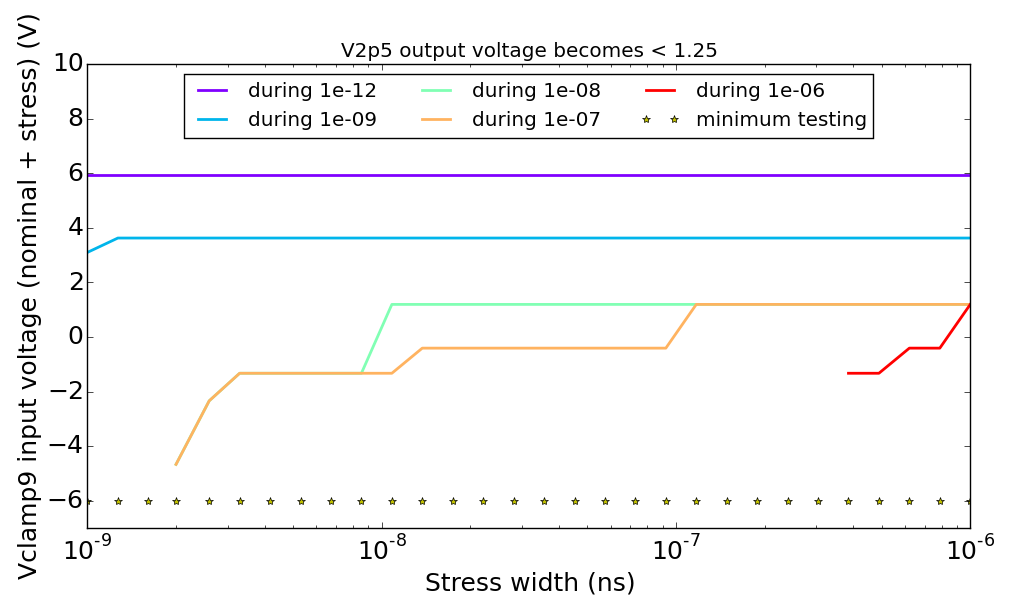
\includegraphics[width=\textwidth]{src/4/figures/cz_bandgap.png}
  \caption{Testchip's bandgap Wunsch & Bell characterization}
  \label{bandgap_wb}
\end{figure}


CURVE CZ REGULATOR

The goal now is to link those curves together, in order to predict if an input
stress applied on the first block can affect the final functionnality outputed
on the last block.

This technique can be done manually.
First, we suppose an ESD stress generated by a 100 ns TLP with a XX V amplitude is injected on the input
of the pre-regulator.

This corresponds on the pre-regulator characterization curve to a point of coordinates (100 ns, XX V).
On the curve, the position of this point shows that in this situation the output of the first block will be at fault (output < X V) for 300? ns.

We can report this output value (X V for 300 ns) on the second curve (bandgap).
The position of this new point means the bandgap will be at fault (below 0V) for 500ns ?

We can repeat again this technique on the third curve (regulator).
The coordinates (0V, 500ns) on the third curve correspond to a regulator at fault (below XX V) during XXXX ns.

In conclusion, using this method, an 100 ns XX V stress on the input of the first block generated a XXXX ns fault on the output of the last block.

The entire process is summarized in fig. X.

ALL THREE CURVES WITH POINT REPORT

To validate it, a full-transistor simulation is run with all three blocks (see Fig. X).
The same 100 ns XX V TLP stress is injected on the same input pin, and the functionnality on the same output pin Y is monitored.
To check the validity of the model, we also monitor voltages at the output of the pre-regulator and the bandgap.

SCHEMATIC FULL CIRCUIT

The simulation of the input, pre-regulator output, bandgap output and final (regulator) output are given fig. X.
On the final output, the complete simulation predicts a much smaller failure than the model.
So there is a large difference between the full simulation and the model.
To try to explain it, intermediates nodes are monitored.

The output of the pre-regulator is below X V (failure criteria) for XX ns in the full simulation while the model predicted XX ns.
Already, at this first block, there is a large difference between the simulation and the model.

The output of the bandgap (second block) shows even a higher difference.
In simulation, the output goes below XX V for XXX ns, while the model predicted XXX ns.

Not only each curve introduces an important error, but errors tend to accumulate after each block.
The origin of this problem needs to be adressed to try to get more accurate results.

SIMULATIONS 2 * 2

Previously, it was indicated that all WnB curves were extracted with a fixed Zout = 1M\textOmega.
In practice, each block (pre-regulator, bandgap, regulator) sees a load impedance on its output much different than that.
Thus, it is important to evaluate the impact of this value on the Wunsch & Bell characterization curve.
The pre-regulator is characterized again, this time with a load impedance of 100\textOmega.
This value is rather small impedance, but sufficiently high to not draw too much current on the pre-regulator.
This second characterization is given fig. X.

CHARACTERIZATION WITH Z LOW IMPEDANCE

This characterization is compared with the one extracted with 1M\textOmega\.
To make the comparison easier, curves for failure above 1ns, 10ns, 100 ns and 1us were plotted separately (see fig. X).
MAKE COMPARISON

COMPARISON Z LOW IMPEDANCE Z HIGH IMPEDANCE 2 * 2 1n -> 1u

SO FAR, CONSIDERED IMPEDANCE AS STATIC AND REAL.
TALK ABOUT IMAGINARY IMPEDANCES, AND DYNAMIC IMPEDANCES

TALK ABOUT ERROR CAUSED BY GRADIENT ?

\subsection{Conclusion regarding bottom-up block failure modeling method}

On paper, this method was rather promising in terms of applicability.
A block could be characterized once, and reused in different places.
The robustness of a full system could have been quickly and easily deduced from the models of its parts.

However, with the study case exposed earlier, several issues arose that clearly limit the ability of the model to perform as expected.

The main issue with this modelling method is the fact that it relies too much
on the value of the output load for performing the characterization of a block.
This load depends on many different parameters.
And this value will change in function out the block connected on the output (think about block-reuse)
Also, this value may not be constant in frequency.
And this value may also not be constant in time (multiple operating modes, biasing points, etc).

Another issue, this method is limited to a binary FAIL/NO FAIL criteria.
Not only this criteria is arbitrary (in some cases, the specification could be used to set it), but
for most purely-analog blocks, there will not be a clear failure, rather, most
nets will have degraded values until maybe biasing of the block completely fails.
In this case, the binary criteria hides a lot of information about the degradation.

ANY CLUES TO OVERCOME THESE ISSUES ?

The main reason why this approach was investigated was for its very interesting modularity
that was highly suitable for block reuse workflow.

However, because of the intrisic interactions between block functions in an integrated circuit,
TRY TO EXPRESS BETTER WHAT PRINCIPLE OF THIS METHOD BOUNDS IT TO FAIL

this approach seems to be bound to fail for building a reusable model for an IC block that could predict
ESD failures at the architecture level and during the IC architecture phase.

\section{Black box modeling approach}

% Difference with bottom-up, not the same application, not the same goal
The black-box modeling method relies on the same core principles than the bottom-up modeling approach.
It studies the relationship and transfert function between the input and the output of a silicon function.
Unlike the bottom-up method though, the model is only built \textbf{for external input and output pins}.
It is not meant to be chained with other models, using a special chaining method.
Instead, it targets electrical, board-level circuit simulations.
Basically, the black box model is intented to act as a drop-in replacement for the complete \gls{ic} circuit, for board-level simulations.

% What is the motivation
%TODO: Reference for SEED
The purpose is also different from the bottom-up approach.
The goal is not to detect issues at silicon-level early before manufacturing, but to let customers using the \gls{ic} in a \gls{pcb} to detect issues with the board that could result in silicon-functions failure.
The \gls{seed} methodology recommends to design systems in a smart fashion for making them robust during operation, which requires a collaboration between board-level and silicon-level protective measures.
Ultimately, the goal is to provide a black box model that is \textbf{fast to simulate} and can be \textbf{distributed without disclosing sensitive intellectual property}.

% introduction, failure relation between input and output
The main benefit of this model is to abstract the internal silicon complexity.
The model focuses on describing the failure of an output when an input is stressed.
At board-level, failure criteria can be more easily set from the chip specification.
After setting the failure criteria, the approach is to inject rectangular pulses on an input pin, and record when an output is in fault.

% access to the signals
Since the characterized nets are external pins, they are physically accessible.
Thus, the black box models can be derived from actual measurements.

\subsection{Failure model}

% How is the characterization conducted
Once again, a variable width/variable amplitude rectangular pulses are applied on an input pin.
The output pin is then observed to detect for which input parameters it is going out of specification.

% What is characterized
This characterization is performed on the testchip, on the complete regulation function.
The characterization pulses are injected on the $V_{batt}$ input.
The output pin is $V_{2p5}$, the regulated supply.
It is supposed to deliver a 2.5V regulated supply.
The failure criteria is set at a voltage below 2.1V.
It corresponds to a level below which digital cells powered by this supply will have noise margins too small for proper operation.

% Fig X shows the waveform of the VBAT injected current when stressed with a TLP (square) impulse.
% The TLP waveform before the capacitor is shown for reference.
%TODO: WAVEFORM CURRENT VBAT AND TLP BEFORE INJECTION CAPACITOR ?

% Detail the characterization
The characterization table is plotted in Fig. \ref{fig:cz-black-box}.
X-axis is the pulse width, and y-axis is the minimal stress amplitude that caused a failure on the output.

\begin{figure}[!h]
  \centering
  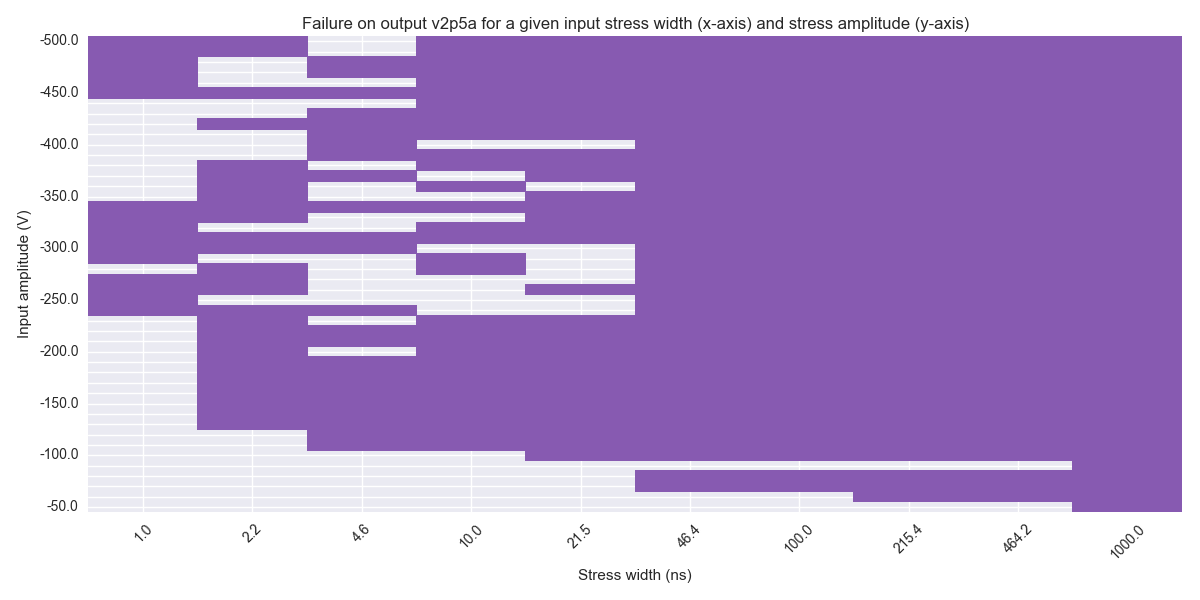
\includegraphics[width=\textwidth]{src/4/figures/black_box_regulator.png}
  \caption{Black-box characterization of the regulation function}
  \label{fig:cz-black-box}
\end{figure}

% What to do with that
%TODO: We that below this value the function is in fail, etc
However, the motivation for this model is to replace the transistor-level schematic inside a SPICE simulation at board-level.
Given a pulse width and an amplitude on $V_{batt}$, the model can estimate the disturbance amplitude and width on $V_{2p5}$.
However, the model itself is not an electrical model, only a failure model.
It cannot determinate, given for instance an input voltage, how much current is flowing into it.
This is also true for the output.
Thus, this method calls for an electrical model of \gls{io}.
The next section details how to solve this issue.

\subsection{Electrical modeling of inputs and outputs}

Need to model a silicon function, between an input external pin and output external pin.
Need an electrical model.
Hypothesis is functions IO can be modeled by their TLP characteristic (quasi-static I(V) response).

In powered or unpowered conditions ?
Unpowered conditions is the simplest, because can be done without external components.
Powered conditions is more challenging, because what to do with external devices ?

First, compare TLP curves on our regulation function, in powered and unpowered conditions.
Not interested in nominal functionnality here, just impedances.
Function does not have to be functionnal, just biased correctly.
Do not connect external devices.

\begin{figure}[!h]
  \centering
  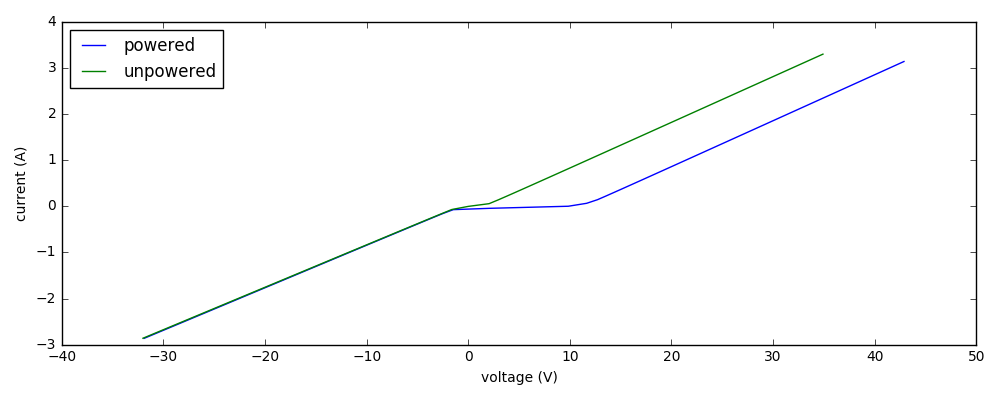
\includegraphics[width=\textwidth]{src/4/figures/tlp_input_characterization.png}
  \caption{TLP characterization of function input in powered and unpowered conditions}
  \label{fig:tlp-input-cz}
\end{figure}

\begin{figure}[!h]
  \centering
  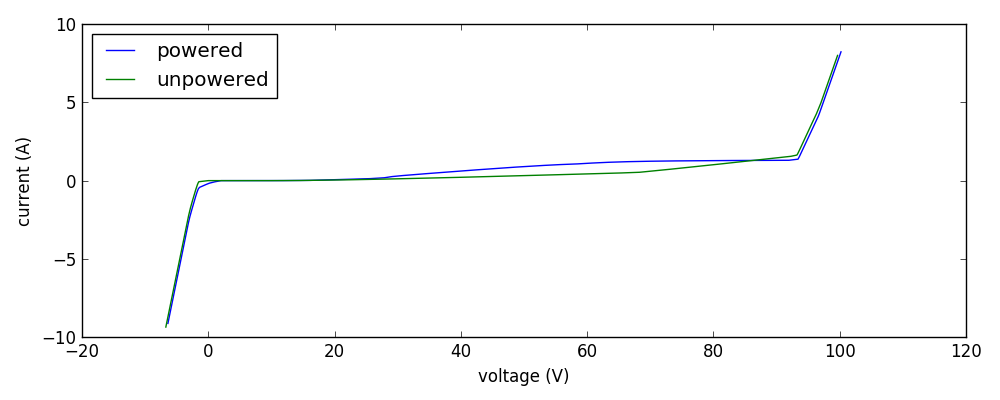
\includegraphics[width=\textwidth]{src/4/figures/tlp_output_characterization.png}
  \caption{TLP characterization of function output in powered and unpowered conditions}
  \label{fig:tlp-output-cz}
\end{figure}

For both input and output, large differences between powered and unpowered modes.
Different amount of current are absorbed by the device in each conditions.
To be as close as possible as the normal testing conditions, characterization should be done in powered conditions.

% Explain the PWL model
Second step to build an electrical model of the function
Create a piecewise linear model of the input, and of the output.
For this purpose, a generic four-points piecewise linear model was written in Verilog-A (TODO: Ref).
Configured with 4 four (V\textsubscript{i},I\textsubscript{i}) points.

\lstset{style=veriloga-style}
\lstinputlisting[caption=Piecewise-linear 4 points model, float, linerange={1-21}, firstnumber=1]{src/4/snippets/pwl_4pts.va}

% Comment the model
Convergence can be difficult to achieve
Must ensure that the PWL is continuous
Also, curves are extracted for a wide range of voltages.
However, it is an integrated function and not an ESD protection.
Thus, any part of the curve beyond the upstream ESD protection triggering-voltage is useless, since voltage will never reach this area.
Also, any part of the curve beyond the Safe-Operating Area (TODO: gloss) of the function is also useless.
Device will be destroyed beyond this limit, in which case we are not interested in functional failures anymore.
Finally, it was observed that rather than trying to fit properly the entire curve with the PWL, it is very important to fit the curve near the nominal voltage.
In our case, between -10V and 40V.


% Validate the model with TLP
Compare full-transistor simulation (nominal + esd) with the input model.
After issues described previously were solved, good agreement is achieved between model and complete circuit, at -10V, 20V and 40V TLP amplitude.
%TODO: Comment waveforms

\begin{figure}[!h]
  \centering
  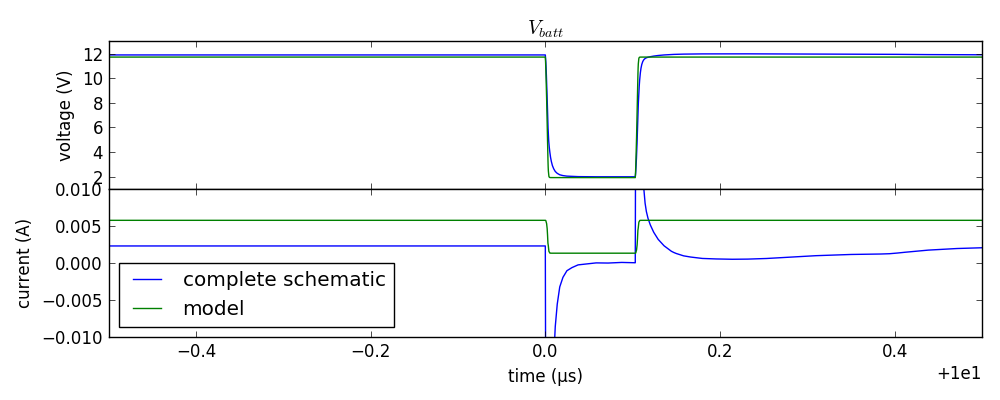
\includegraphics[width=\textwidth]{src/4/figures/comparison_model_total_m10V.png}
  \caption{Comparison of complete schematic and model simulations - -10V TLP}
  \label{fig:compare-model-simu-m10}
\end{figure}

\begin{figure}[!h]
  \centering
  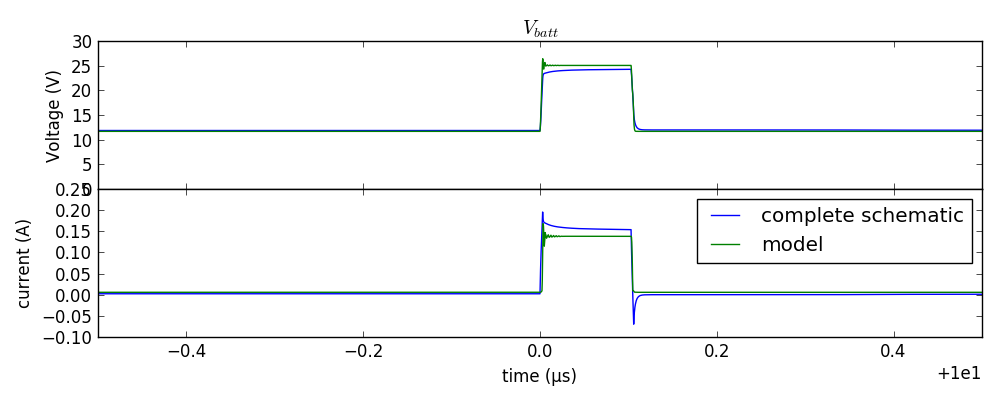
\includegraphics[width=\textwidth]{src/4/figures/comparison_model_total_20V.png}
  \caption{Comparison of complete schematic and model simulations - 20V TLP}
  \label{fig:compare-model-simu-20}
\end{figure}

\begin{figure}[!h]
  \centering
  \includegraphics[width=\textwidth]{src/4/figures/comparison_model_total_40V.png}
  \caption{Comparison of complete schematic and model simulations - 40V TLP}
  \label{fig:compare-model-simu-40}
\end{figure}

%TODO: Move as opening ?
Also, need to validate with a varying waveform

\subsection{Combining failure and electrical models}

% What is the complete model
The complete function model combines the input piecewise-linear model, the failure model, the output piecewise-linear model, and an output DC source (for settling nominal value).

Fig. \ref{fig:complete-black-box-model}
The failure model act as a voltage-controlled voltage source, controlled by the input, and acting on the output.
Given an disturbance amplitude and width and width on the input, it configures and generates a rectangular pulse on the output.

\begin{figure}[!h]
  \centering
  \includegraphics[width=0.3\textwidth]{src/4/figures/complete_black_box_model.pdf}
  \caption{Architecture of the complete black-box model}
  \label{fig:complete-black-box-model}
\end{figure}

% how is this model
To test the entire concept, two simulations are run.
The first one is the classic, transistor-level simulation of the function exposed to a (XX V, XXX ns) disturbance.
It serves as a reference.
The second simulation simulates only the output of the model.
The output failure source generates a rectangular pulse of (XXX V, XXX ns), corresponding to the same (XX V, XXX ns) disturbance on the input than the reference.
The goal is to verify if the model can reproduce even partially the disturbance on the output pin.

%TODO: Simulation

In conclusion, it can reproduce the variation on the output, for a given input disturbance.

\subsection{Conclusion on black-box modeling}

% Conclusion
Black box models of analog integrated functions are very interesting for distributing SPICE models to external parties.
They do not disclose the internal design of the chip, yet they can help achieve system-level ESD simulations.
Ultimately, the goal is to follow the SEED (TODO: Ref) methodology, that indicates that ESD robustness should not be handled at a single level of a system, but at every level (equipment, board, integrated circuit), and that all levels should work efficiently together toward that goal.
Black box models fit very nicely in this methodology.
In this section, a first technique for extracting and creating black-box models was presented.
There is a lot of room for improvements, but it is already working for some intermediate complex cases.
The core principle is that TLP characterization of inputs and ouputs on a biased function is sufficient to extract an equivalent impedance.
This impedance can replace the function in the schematic, during an ESD simulation, in order to reduce complexity and simulation time.
The second core principle is to simplify waveforms into rectangular ones in order to reduce the complexity of the problem.

% Opening work
There are many new leads to explore on these black box models.
First, behavior of the models against more time-varying disturbances such as ESD gun waveforms should be investigated.
Also, the piecewise-linear models should be improved to be more stable, and to fit more closely the extracted I(V) curve.
This technique should be applied to a wider number of analog functions, to observe if it can be used in a general manner.
For now, input and outputs must be simulated separately.
First, the input is simulated, then analyzed to extract the width and amplitude of the disturbance.
This data is then used to configure the output failure source pulse.
The model must be improved in order for the output to react in real-time to the disturbance of the input.
Ultimately, this calls for a Verilog-A model of the failure for instance, plus most likely an improved characterization method able to extract and describe this real-time behavior.

\section{Blabla}

%\section{Application of Wunsch & Bell curves to arbitrary waveforms}
\label{sec:wb-for-arbitrary-wvfs}

% WB here based on amplitude/duration of square pulse
WB

% Reality is more arbitratry, time varying pulse

\subsection{Integration method}

% Explain what this method is
Integration

\subsection{Amplitude-distribution method}

% Explain what this method is
Distribution


% End of chapter files listing

% Conclusion
\chapter{Conclusion}
\label{sec:final-conclusion}

As presented in the introduction, ESD are a major source of stress for electronic devices.
They can cause hardware failures, damaging permanently devices.
This class of issues has been studied for many years, and is the core of ESD research.
Recently, a new class of failures started to be considered.
Electrostatic discharges can cause temporary disturbances on devices.
In the context of always ever-more sensitive electronic devices and IC in particular, this is an issue.
Even more considering that electronic modules nowadays have increasingly large responsabilities in regard of our safety.
New trends for the autonomous car ask electronics to take vital decisions such as braking, direction, etc.
Guarantying safety of operation against electrostatic discharge is critical.

% Chap 1
In a first phase, a review of the test methods common in the ESD field was conducted, to identify relevant and realistic stress sources in laboratory environment.
Then, a review of the litterature on soft-failure analysis and prediction method showed few research at silicon level.
Many general-purpose observation techniques exist such as EMMI, Near-field scan.
Simulation tools were used in the past, such as \gls{spice} simulation of course, and more advanced techniques such as 3D full-wave electromagnetic simulations or \gls{tcad} simulations.
These tools are highly interesting at the system and board level, to evaluate what fraction of an incoming discharge actually reach an integrated circuit.
We were interested in electrical simulations of conducted disturbances in particular.

% Chap 2
For this purpose, chapter 2 provides a detailed modelling method of electronic systems for ESD that relies on past work on the topic.
A modular approach is adopted, where each component is modelled individually to form a library, then assembled together in a hierarchical fashion.
Mostly physically based and most parameters can be extracted with simple tools, or by estimatation where it is sometimes enough.
A concrete case study is presented with the modelling of a complex TLP generator.
It is perfect to illustrate a few key points for the modelling methods, and to demonstrate its accuracy against a lot of reference measurements.

% TLP-HMM
The development of this model and the insights gained in the process led to the development of a new pulse generator.
It reproduces the HMM waveform, one of the most widely used test pulse in the ESD field, but in a shielded and controlled environment.
The benefits are increased reproducibility of testing results and a flexibility for shaping the pulse waveform.
The prototype helped identified early issues and improvement to make.

% Correlation method
When comparing this generator to actual ESD guns and standard TLP, a new correlation method has been discovered.
It was validated successfully on 10 different ESD protections.
Correlation methods between ESD generators are extremely valuable because they can ultimately reduce testing time.
By testing a part with a single generator it is possible to predict the failure levels found with the others.
Before being able to do so, the correlation method should be tested on a much larger set of ESD protection.
Failure analysis on the destroyed parts should be conducted to verify if the failure mechanism remains identical between the different generator.

% Near-field current processing
In the last part of the chapter 2, a detailed post-processing method for on-chip near-field sensor has been presented.
It details the operation of the post-processing pipeline developped for this kind of sensor.
The processing script is released \cite{} under an open-source license in order to promote collaboration and future improvements on the topic.
Two different methods are evaluated and compared in order to reconstitute a current waveform from the voltage measured accross the on-chip sensor.

% Chap 3
Chapter 3 is a direct application on-silicon of those investigation methods.
An actual case study is presented, where a complex analog function restarts because of an ESD.
The function is a primary regulator for a large automotive product.
To gain more insights and data, a custom test vehicle has been designed.
Some monitoring structures were designed specifically for this purpose.
Not all monitoring techniques were successfull, as a few issues were met with the communication system responsible for outputting some measurement data.
Those issues can be fixed for future testchips.
Overall, the on-chip monitoring method lays a ground work for future silicon-level research and could be reused.

% Chapter 4
Research work also focused on developping tools for simulation environment.
This work is presented in chapter 4.
The value of simulation tools is well known, because it enables to detect issues very early in the development cycle, which is extremely valuable for avoiding late issues and cutting the cost of fixing them late.
The main challenge for ESD at silicon-level is the complexity of the circuits and simulations.
Convergence issues are very common and sometimes extremely difficult to avoid.
The complexity of the circuits makes finding issues manually extremely hard.
Most of the time, it is required to manufacture a first silicon to test the parts against ESD and identify soft-failures.
To avoid those issues, new methods are required and two of them were proposed and explored during this research.

% First modelling method
The first method consist in characterizing and modelling some blocks of an analog function.
More specifically, the relationship between a given block input and block output.
Goal is to know at the silicon level what individual block was disturbed.
It is definitely a tool for the IC designers.
After a block model was constructed, it is possible to propagate from block to block a disturbance in the shape of a rectangular pulse of a given width and amplitude.
After each block, the disturbance changes, can increase or decrease in amplitude, become longer or shorter.
Ultimately, this method gives a "bounding box" of the disturbance on the final net, which is often sufficient to detect a functional failure.
This approach was tested with some success on the same case study than put previously on silicon.
It is still at its very early days, assumes a lot of simplifications and requires many improvements, however preliminary results tend to show it could actually be usable in a foreseeable future.
There are several challenges to overcome, in particular identifying the proprer level in the hierarchy to model the blocks.
Also, the propagation path is considered unidirectionnal, the discharge propagates from an entry point to an outer point.
It is not really realistic, because it fact it spreads around the circuit.
However, it is important to make simplifications initially in order to get a prototype at work and evaluate what improvements or modifications are actually needed.

% Second modelling approach
The second modelling method is more focused on facilitating cooperation between IC manufacturers and equipment manufacturers.
It integrates well inside the SEED methodology, where interaction between these two actors helps design robust products against ESD with optimal cost and development time.
The objective is to characterize and model the relationship between an input pin and an output pin, and to check if a board simulation can be conducted with this black-box IC model.
It was shown that a TLP characterization constitutes a good base for a pin model, in particular for modelling inputs.
For output pins that are supposed to drive a potential in DC conditions, it was demonstrated that this method does not work and requires modifications.
The I(V) curve extracted with the TLP combined with a DC model fails to drive correctly the output voltage and current.
It is an interesting result that calls for more research on this topic.

% Proposal
Finally, a new method is proposed for IC design teams.
It is a complete proposal and has not been tested so far, however the concept seems highly promising with implications much further than ESD powered-on analysis and prediction.
The idea is to let analog designers define for their analog function blocks a set of assertions, or checks, that are mandatory for proper operation.
For instance, the check could be to ensure that a large enough voltage difference is present between the gate of a current mirror and ground.
It is also possible to add a check to ensure that a ground net never goes above a few hundred millivolts, otherwise it is either the sign that an ESD has induced a ground shift or that this net is simply floating.
Ultimately, each block could own its set of functional assertions, that would be checked by the simulator.
An appropriate tooling for observing the results and failed assertions is of course required, but it would be extremely helpful during power-on esd analysis to find which block was at fault, what block failed the first, understand how a disturbance has propagated inside the circuit and much more.
This tool could serve during the normal design flow, to guarantee functionality and immediately detect issues in block interconnections for instance.
There are no known technology locks that would present this method to be implemented.
Although not tested due to a lack of time, this tool is proposed and described inside this document because it was imagined from the experience gained with this research, and is believe to yield good and positive results.
Because of its modular nature (each block gets its own set of assertions), it fits extremely well inside the current IC design flow.
In particular, it is very friendly for modular IC design trends such as IP block reuse.
There are many challenges, in terms of user interaction, processing and display of results, integration with current simulation environments to be solved.
A first prototype could serve as a ground work to identify more accurately those challenges and prepare for a more advanced implementation.

% Final Conclusion
In conclusion, this work has explored many different topics and axes in the relatively new field of soft-failure ESD analysis.
The research could have been conducted in a very different manner.
For instance, it could have been a lot more IC-design-oriented.
A specific failure could have been studied extensively, a patch proposed and tested with a test-vehicle.
However, it was decided that this kind of highly specific highly focused approach would not be beneficial for future work.
Instead, more general methods and tools were explored.
At the end of this work, most of them remain merely at the prototyping phase.
We feel that this work provided new axes and research for future research, and that other people can actually takes those tools from a prototype to a production ready tool.
Improvements to near-field scan processing, improvements of the TLP-HMM and a larger validation of the TLP versus HMM correlation are probably the most simple follow-up work on the topic.
The bottom-up modelling method, the black-box IC method are still largely at the prototype phase and will require extensive research work before being production-ready.
Finally, the functional block checker, probably the most promising method among all those explored, needs initial work to make a prototype and evaluate the concept.

% Appendix
\begin{appendices}
\chapter{Testchip register maps}
\label{apx:testchip-register-maps}

Read chain 1
Index	Bit	Function
0	v2p5d	input connected to v2p5 - should always be 0b1
1	agnd	input connected to agnd - should always be 0b0
2	vdd	level down shifter sampling an 8V reference - should always be 0b1
3	agnd	level down shifter sampling agnd - should always be 0b0
4	ov	test_A : raw OV output
5	uv	test_A : raw UV output
6	ov_2p5	test_A : raw_OV output with 2p5 static ref
7	ov_4p9	test_A : raw_OV output with 4p9 static ref
8	ov_5p0	test_A : raw_OV output with 5p0 static ref
9	ov_5p1	test_A : raw_OV output with 5p1 static ref
10	ov_7p5	test_A : raw_OV output with 7p5 static ref
11	ov_0MHz	test_B : raw OV output without filter
12	ov_20MHz	test_B : raw OV output with 20MHz lpf
13	ov_10MHz	test_B : raw OV output with 10MHz lpf
14	ov_5MHz	test_B : raw OV output with 5MHz lpf
15	ov_2MHz	test_B : raw OV output with 2MHz lpf
16	ov_1MHz	test_B : raw OV output with 1MHz lpf
17	ov_0kHz	test_C : raw OV output without filter
18	ov_500kHz	test_C : raw OV output with 500 kHz lpf
19	ov_200kHz	test_C : raw OV output with 200 kHz lpf
20	ov_100kHz	test_C : raw OV output with 100 kHz lpf
21	ov_50kHz	test_C : raw OV output with 50 kHz lpf
22	ov_20kHz	test_C : raw OV output with 20 kHz lpf
23	agnd	input connected to agnd - should always be 0b0
24	v2p5d	input connected to v2p5 - should always be 0b1


Write chain 1
Index	Bit	Function
0	D_pout<0>	Writes 0b0 or 0b1 on pin
1	D_pout<1>	Writes 0b0 or 0b1 on pin
2	D_pout<2>	Writes 0b0 or 0b1 on pin
3	D_pout<3>	Writes 0b0 or 0b1 on pin
4	ref<0>	test_D : tunable reference : MSB - active low
5	ref<1>	test_D : tunable reference : bit 2 - active low
6	ref<2>	test_D : tunable reference : bit 3 - active low
7	ref<3>	test_D : tunable reference : bit 4 - active low
8	ref<4>	test_D : tunable reference : bit 5 - active low
9	ref<5>	test_D : tunable reference : bit 6 - active low
10	ref<6>	test_D : tunable reference : LSB - active low


Read chain 2
Index	Bit	Function
0	vdd_nuv
1	vdd_nuv_deg	test_vdd_nuv_deglitch
2	v2p5_nuv	test_v2p5_nuv
3	v2p5_nuv_deg
4	uv_9V_div4	uv_vclamp9_div4
5	ov_9V_div4	ov_vclamp9_div4
6	ov_vref1p2	ov_vref1p2_bg1
7	ov2p5_1p2	ov2p5_vref1p2_bg1
8		uv_5MHz_vclamp9_div4
9		uv_200kHz_vclamp9_div4
10		ov_5MHz_vclamp9_div4
11		ov_200kHz_vclamp9_div4


Write chain 2
Index	Bit	Function
0	vref_uv_9V	MSB
1
2
3
4
5
6		LSB
7	vref_ov_9V	MSB
8
9
10
11
12
13		LSB
14	vref_1p2	MSB
15
16
17
18
19
20		LSB

\chapter{TLP modeling}
\section{Validation curves}
\label{apx:tlp-validation-curves}

\begin{figure}[!h]
  \centering
  \includegraphics[width=\textwidth]{src/2/figures/tlp_comparison_open_10V.png}
  \caption{Voltage and current waveforms comparison : 10 V charging voltage on open circuit}
  \label{fig:comparison-tlp-open-10v}
\end{figure}

\begin{figure}[!h]
  \centering
  \includegraphics[width=\textwidth]{src/2/figures/tlp_comparison_open_1000V.png}
  \caption{Voltage and current waveforms comparison : 1000 V charging voltage on open circuit}
  \label{fig:comparison-tlp-open-1000V}
\end{figure}

\begin{figure}[!h]
  \centering
  \includegraphics[width=\textwidth]{src/2/figures/tlp_comparison_short_10V.png}
  \caption{Voltage and current waveforms comparison : 10 V charging voltage on a short circuit}
  \label{fig:comparison-tlp-short-10V}
\end{figure}

\begin{figure}[!h]
  \centering
  \includegraphics[width=\textwidth]{src/2/figures/tlp_comparison_short_1000V.png}
  \caption{Voltage and current waveforms comparison : 1000 V charging voltage on a short circuit}
  \label{fig:comparison-tlp-short-1000V}
\end{figure}

\begin{figure}[!h]
  \centering
  \includegraphics[width=\textwidth]{src/2/figures/tlp_comparison_R25_10V.png}
  \caption{Voltage and current waveforms comparison : 10 V charging voltage on 25\textOmega{}}
  \label{fig:comparison-tlp-load-10v}
\end{figure}

\begin{figure}[!h]
  \centering
  \includegraphics[width=\textwidth]{src/2/figures/tlp_comparison_R25_1000V.png}
  \caption{Voltage and current waveforms comparison : 1000 V charging voltage on 25\textOmega{}}
  \label{fig:comparison-tlp-load-1000v}
\end{figure}

\begin{figure}[!h]
  \centering
  \includegraphics[width=\textwidth]{src/2/figures/tlp_comparison_470nH_500V.png}
  \caption{Voltage and current waveforms comparison : 500 V charging voltage on a 470nH inductor}
  \label{fig:comparison-tlp-inductor}
\end{figure}

\chapter{Bottom-up block characterization and modeling}
\section{Characterizations}
\label{apx:block-cz}

\begin{figure}[!h]
  \centering
  \includegraphics[width=\textwidth]{src/4/figures/bandgap_cz_v2_amplitude.png}
  \caption{Bandgap V\textsubscript{clamp9} amplitude matrix}
  \label{fig:bg_amp}
\end{figure}

\begin{figure}[!h]
  \centering
  \includegraphics[width=\textwidth]{src/4/figures/bandgap_cz_v2_width.png}
  \caption{Bandgap V\textsubscript{clamp9} width matrix}
  \label{fig:bg_width}
\end{figure}

\begin{figure}[!h]
  \centering
  \includegraphics[width=\textwidth]{src/4/figures/regulator_cz_v2_amplitude.png}
  \caption{Regulator V\textsubscript{clamp9} amplitude matrix}
  \label{fig:regu_amp}
\end{figure}

\begin{figure}[!h]
  \centering
  \includegraphics[width=\textwidth]{src/4/figures/regulator_cz_v2_width.png}
  \caption{Regulator V\textsubscript{clamp9} width matrix}
  \label{fig:regu_width}
\end{figure}

\section{Improved model chain versus reference}
\label{apx:block-model-comparison}

\begin{figure}[!h]
  \centering
  \includegraphics[width=\textwidth]{src/4/figures/total_simulation_20V_100n_V2.png}
  \caption{Reference versus model chain waveforms for a \SI{-20}{\volt} \SI{100}{\nano\second} stimulus}
  \label{fig:reference_simu_v2_20V_100n}
\end{figure}


\begin{figure}[!h]
  \centering
  \includegraphics[width=\textwidth]{src/4/figures/total_simulation_20V_1u_V2.png}
  \caption{Reference versus model chain waveforms for a \SI{-20}{\volt} \SI{1}{\micro\second} stimulus}
  \label{fig:reference_simu_v2_20V_100n}
\end{figure}

\end{appendices}


% Bibliography
\bibliographystyle{unsrt}
\bibliography{../src/refs}
\printindex

% List of code snippets
\listoflistings

% Glossary
\setglossarystyle{altlist}
\printglossaries

\end{document}
